\documentclass[notitlepage, twocolumn]{article}

\usepackage[left=0.6in, right=0.6in, top=0.8in, bottom=0.8in]{geometry}
\usepackage{titling}
\usepackage[compact]{titlesec}
\usepackage{lipsum}
\usepackage{graphicx}
\usepackage[labelfont=bf, labelsep=space, font=small]{caption}
\usepackage[labelformat=simple]{subcaption}
\usepackage[noabbrev]{cleveref}
\usepackage{mwe}
\usepackage{sansmathfonts}
\usepackage{amsmath}
\usepackage{float}
\usepackage{fancyhdr}
\usepackage{cite}
\usepackage{multicol}
\usepackage{booktabs}
\usepackage{stfloats}
\usepackage{hyperref}
\usepackage[flushleft]{threeparttable}
\usepackage[noblocks, affil-it]{authblk}
\usepackage{enumerate}

\pagestyle{fancy}
\fancyhf{}
\fancyhead[LE,RO]{}
\fancyhead[RE,LO]{}
\fancyfoot[CE,CO]{}
\fancyfoot[LE,RO]{\thepage}
 
\renewcommand{\headrulewidth}{0.5pt}
% \renewcommand{\footrulewidth}{0.5pt}

% set fonts
\renewcommand{\familydefault}{\sfdefault}
\captionsetup[figure]{font={sf, small}}

\titleformat*{\section}{\large\bfseries\uppercase}
\titleformat*{\subsection}{\bfseries}

\titlespacing*{\section}{0pt}{\baselineskip}{1pt}
\titlespacing*{\subsection}{0pt}{0.5\baselineskip}{1pt}

\renewcommand{\abstractname}{\vspace{-\baselineskip}} % Remove Abstract header

\newcommand\invisiblesection[1]{%
  \refstepcounter{section}%
  \addcontentsline{toc}{section}{\protect\numberline{\thesection}#1}%
  \sectionmark{#1}\phantom{}}

\newcommand{\specialcell}[2][c]{%
  \begin{tabular}[t]{@{}c@{}}#2\end{tabular}}

\DeclareCaptionFormat{myformat}{#1#2#3\hrulefill}
\DeclareCaptionLabelFormat{bold}{\textbf{#2}}
\captionsetup[figure]{format=myformat, subrefformat=bold}
\captionsetup[subfigure]{format=default}

\pretitle{\Huge}
\posttitle{\par\vskip 0.5em}
\preauthor{\bfseries}
\postauthor{}
\predate{\par\large\centering}
\postdate{\par}

\title{Unified variation discovery and genotyping from high-throughput sequencing data}

\author[1,2,*]{Daniel Cooke}
\author[2]{David Wedge}
\author[1]{Gerton Lunter}
\affil[1]{\footnotesize Wellcome Centre for Human Genetics, University of Oxford, Oxford, UK}
\affil[2]{\footnotesize Big Data Institute, University of Oxford, Oxford, UK}
\affil[*]{\footnotesize Correspondence should be addressed to D.C (dcooke@well.ox.ac.uk)}

\date{}

\begin{document}

\maketitle

\thispagestyle{empty}

\begin{abstract}\textbf{
Haplotype-based variant callers, which consider physical linkage between variation sites, are currently the \textit{de facto} choice for germline variation discovery and genotyping. However, there are few established haplotype-based tools beyond those aimed at detecting common germline variation in diploid individuals. Here we present Octopus, a flexible haplotype-based variant caller that employs a polymorphic Bayesian genotyping model that may be engineered for a range of experimental designs. Octopus is more accurate than existing germline, somatic, and \textit{de novo} mutation detection tools; is able to call a wide range of variation, including microinversions and complex replacements; includes a probabilistic phasing algorithm that is able to phase arbitrary ploidy genotypes and somatic mutations; outputs realigned evidence BAM files to aid validation; and is readily extendible to atypical samples and new sequencing technology.
}\end{abstract}

\invisiblesection{Motivation}

Haplotype-based variant callers have emerged as the method of choice for calling germline variants because they alleviate alignment errors from read mappers and have better signal-to-noise characteristics than positional approaches \cite{RN5, RN604, RN562, RN141, RN538, RN598, RN166}. However, existing haplotype-based tools have several limitations. First, existing tools are suboptimal for many problems as most only implement genotype likelihood models that assume either diploid \cite{RN5, RN604, RN562} or constant \cite{RN141, RN538, RN598} ploidy and copy number, and genotype prior models that assume samples are selected from an idealised population with unknown relatedness. Such models are well suited to calling germline variants in small cohorts, but offer a poor fit to data typically generated from other other experimental designs where the number and frequency of haplotypes is unknown, such as in tumour or bacterial sequencing, or when sample relatedness is known, such as when calling a tumour-normal pair or parent-offspring trios. This limitation means researchers with bespoke requirements often resort to custom pipelines that may integrate various callers and involve \textit{post hoc} filtering and interpretation \cite{RN156, RN361, RN373, RN276, RN3, RN514, RN541, RN540}. Second, existing haplotype-based methods suffer \emph{window artefacts} as variation is evaluated in independent non-overlapping \emph{active regions}. This can lead to false calls in complex regions where reads support variation that is not in the active region. Third, existing methods do not make a clear distinction between the haplotype sequence supported by the read data, and the mutation events that gave rise to it. This makes it challenging to assign appropriate prior probabilities to these haplotype sequences, because different sets of mutation scan have very different biological plausibility, despite giving rise to the same haplotype sequence. Fourth, despite haplotype-based methods being able to physically phase variants, phasing algorithms are currently limited to diploid genotypes, therefore no tool currently reports phase information for somatic mutations, which can have important consequences for disease \cite{RN211}.

To meet the growing demand for variant calling in disparate experimental designs, we designed an algorithm that can accomodate distinct genotype models within a unified haplotype-aware framework. We took inspiration from particle filtering \cite{Doucet11atutorial} and developed a novel haplotype inference procedure that typically produces longer haplotypes than other methods, reducing the chance of window artefacts and improving the signal-to-noise ratio, leading to better calling accuracy. Furthermore, our method can propose and compare haplotypes with identical sequence, but distinct composing mutation events, allowing us to consider the biological plausibility of mutations. We propose a probabilistic phasing algorithm that leverages both prior and read information, and can phase genotypes with arbitrary ploidy, including those that contain somatic mutations - a first to our knowledge. 

We present an implementation of our algorithm, \emph{Octopus}, written in C++. We show Octopus is more accurate than specialised tools on several common use-cases: germline callling in individuals, \textit{de novo} calling in parent-offspring trios, and somatic variant calling in paired and unpaired tumours. Octopus 

Octopus is freely available under the MIT license at \url{https://github.com/luntergroup/Octopus}.

\section*{Results}

\subsection*{Calling variants from biologically distinct data sources}

\begin{table}[ht]
    \centering
    \small
    \sffamily
    \caption{Description of Bayesian calling models}
    \label{table:calling_models}
    \resizebox{\columnwidth}{!}{%
	\begin{threeparttable}
    \begin{tabular}{@{}p{0.2\linewidth}p{0.15\linewidth}p{0.65\linewidth}@{}}
        \toprule
        Model name & Class & Description \\
        \midrule
        Individual* & Germline & Call germline variation in an individual with known ploidy. Haplotypes are expected to be observed at a frequency proportional to their copy number. \\
        \addlinespace
        Population & Germline & Jointly call germline variation in two or more samples with known ploidy but unknown relationship. Uses a joint genotype prior which can improve power to detect variation compared with individual calling by sharing information across samples. \\
        \addlinespace
        Trio* & \specialcell{Germline\\\textit{De novo}} & Jointly call inherited and \textit{de novo} germline variation in a diploid parent-offspring trio. By explicitly modelling inheritance patterns and \textit{de novo} mutations, the model has better power compared with typical joint calling. Allosome calling is supported. \\
        \addlinespace
        Cancer* & \specialcell{Germline\\Somatic} & Jointly call germline and somatic variation in paired tumour-normal or tumour only samples. The number of somatic haplotypes and their frequency are inferred from the data and used to call variants. Multiple tumours from the same individual may be called jointly. \\
        \addlinespace
        Polyclone & Germline & Call variation in an unknown mixture of haploid clones. Such samples often arrise in bacterial or viral sequencing data where multiple clones may form due to sample contamination, mixed infection, or in-host evolution. The model infers the number of haplotypes and their frequency using Bayesian model comparison. \\
        \bottomrule
    \end{tabular}
	\begin{tablenotes}
	      \small
	      \item * Evaluated in this article.
	    \end{tablenotes}
	\end{threeparttable}
    }
\end{table}

Octopus accepts sequencing data in the BAM/CRAM format, and performs internal pre-processing, including PCR duplicate filtering and downsampling. Candidate variants are detected from the reads using local re-assembly and pileup inspection. Variants from external sources may also be considered. Haplotypes are then constructed exhaustively using a tree-based data structure (nodes are alleles and branches haplotypes) that is dynamically pruned, extended, and collapsed based on partially observed evidence. Only once there is confidence the haplotypes in the tree explain all surrounding reads are calls made. Haplotype likelihoods are computed for each read and haplotype using a hidden Markov Model (HMM) with context aware SNV and indel penalties. These likelihoods are the input to a polymorphic genotype \emph{calling model}, the form of which depends on experiment that generated the sequencing data (Table \ref{table:calling_models}). Although each calling model is responsible for calling variants, genotypes, and any other model specific inferences, each must be able to compute a posterior distribution over haplotypes and genotypes, which are used for updating the haplotype tree and for phasing respectively. Variants are phased by evaluating the entropy of the computed genotype posterior distribution. Variant calls are then filtered, either with hard filters or a random forest classifier. Octopus optionally creates realigned evidence BAMs after calling by assigning reads to called haplotypes. For a more detailed discussion of each step of the algorithm see the \textbf{Methods}.

\subsection*{Germline variants from WGS}

\begin{figure*}[ht!]
    \centering
    \vspace{-0.5cm}
\captionsetup[subfigure]{position=top,labelfont=bf,textfont=normalfont,singlelinecheck=off,justification=raggedright}
    \begin{subfigure}[b]{\textwidth}
        \caption{}
        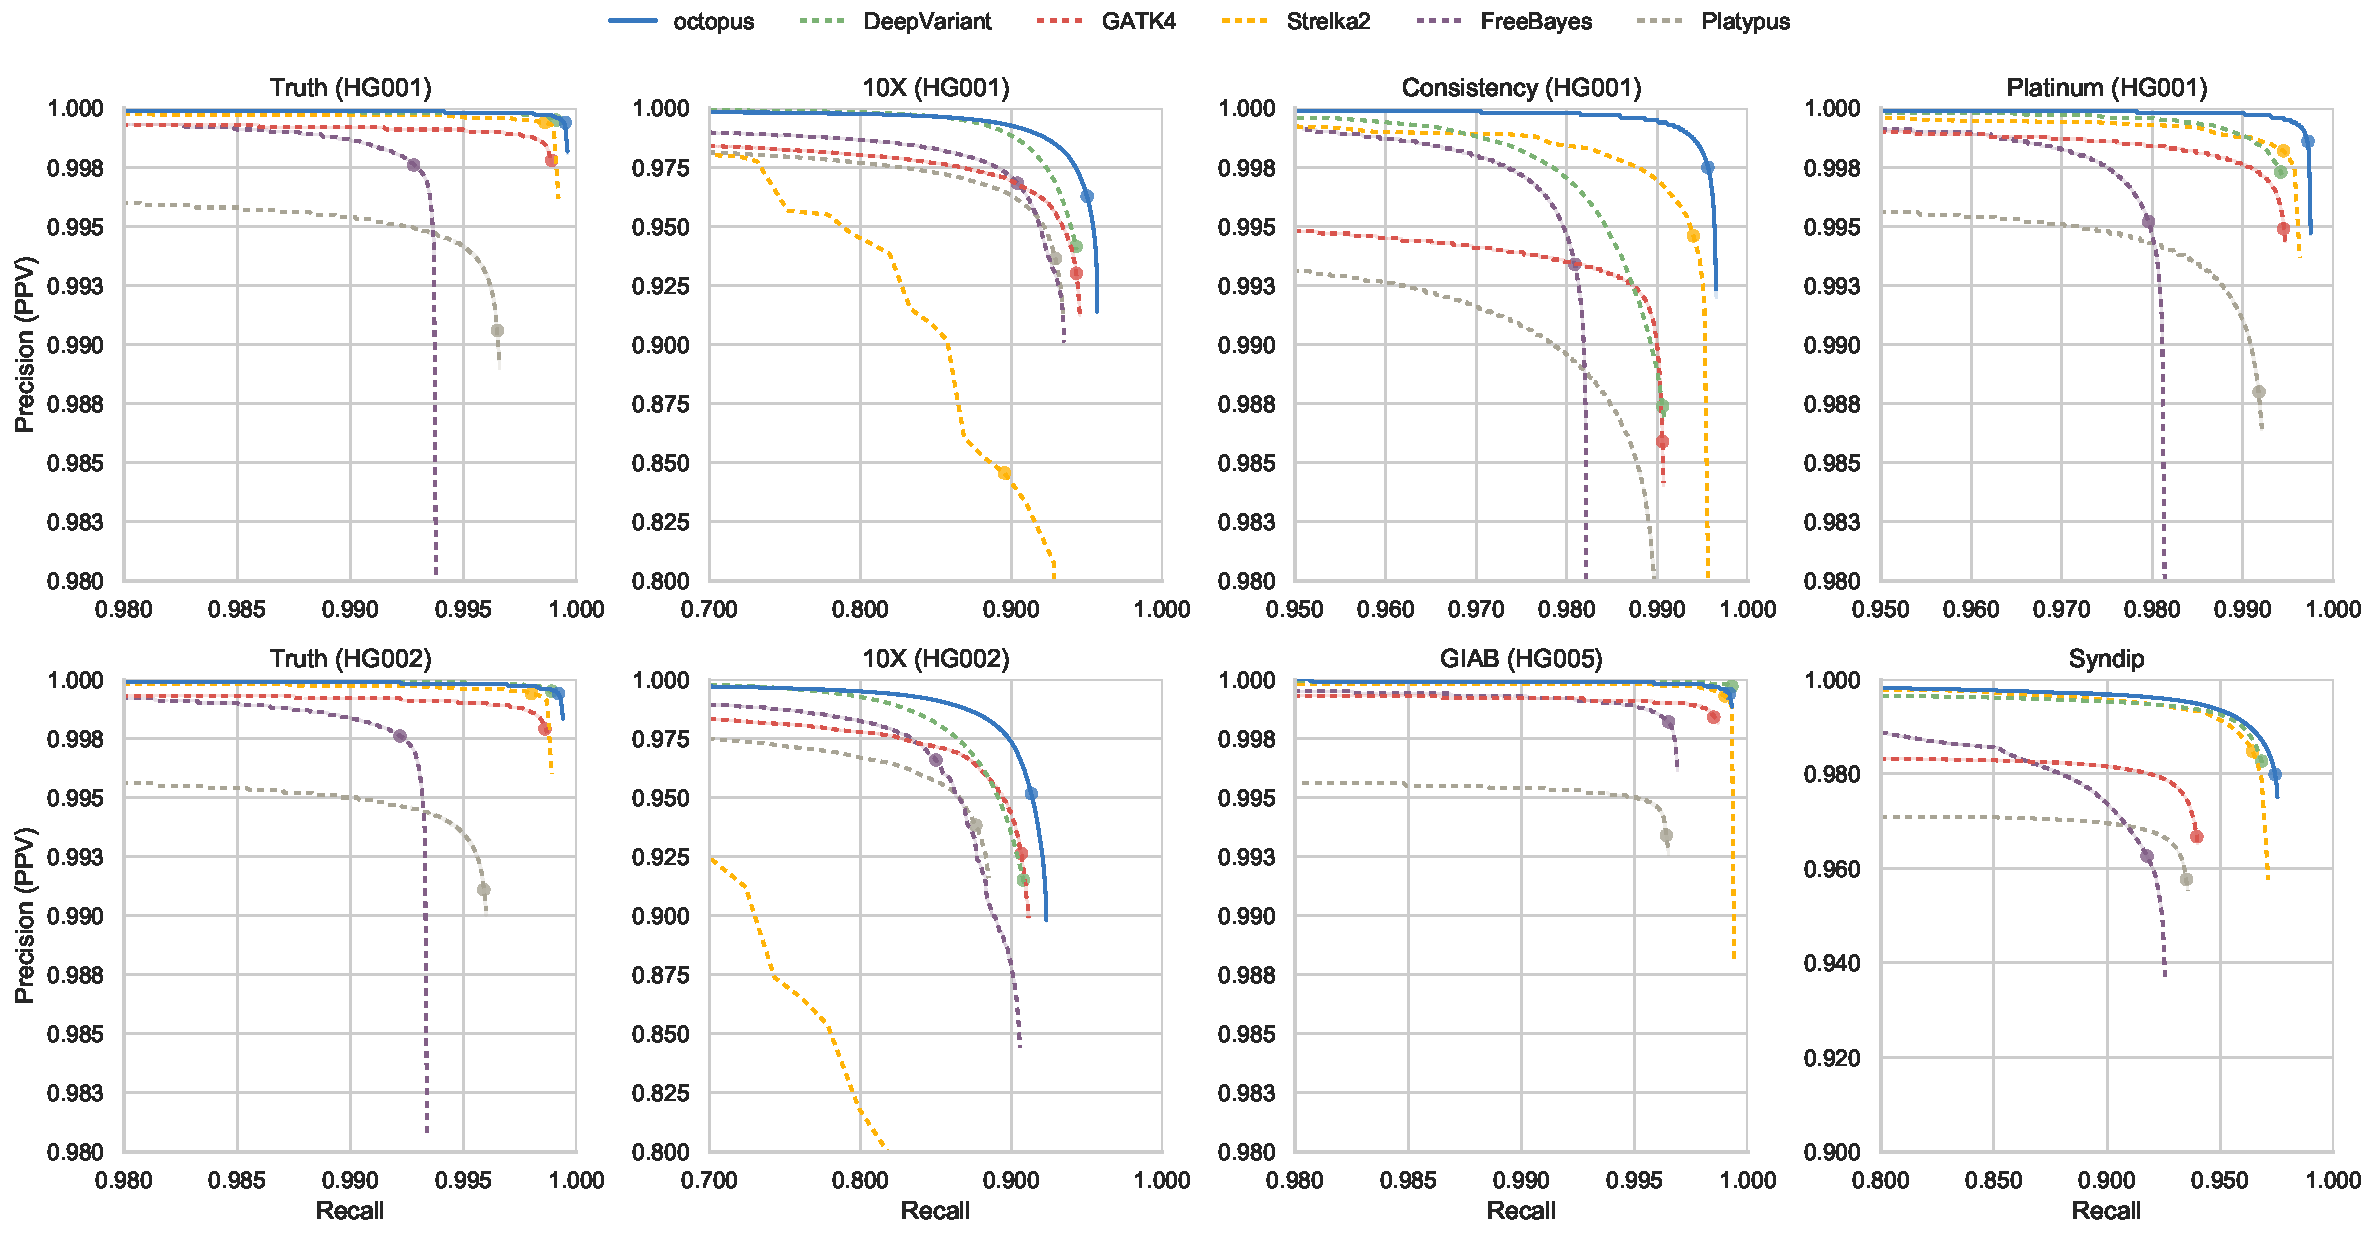
\includegraphics[width=\textwidth]{figures/germline_precision_recals}
        \label{fig:germline:precision-recall}
    \end{subfigure}
    \begin{subfigure}[b]{0.49\textwidth}
        \vspace{-0.5cm}
        \caption{}
        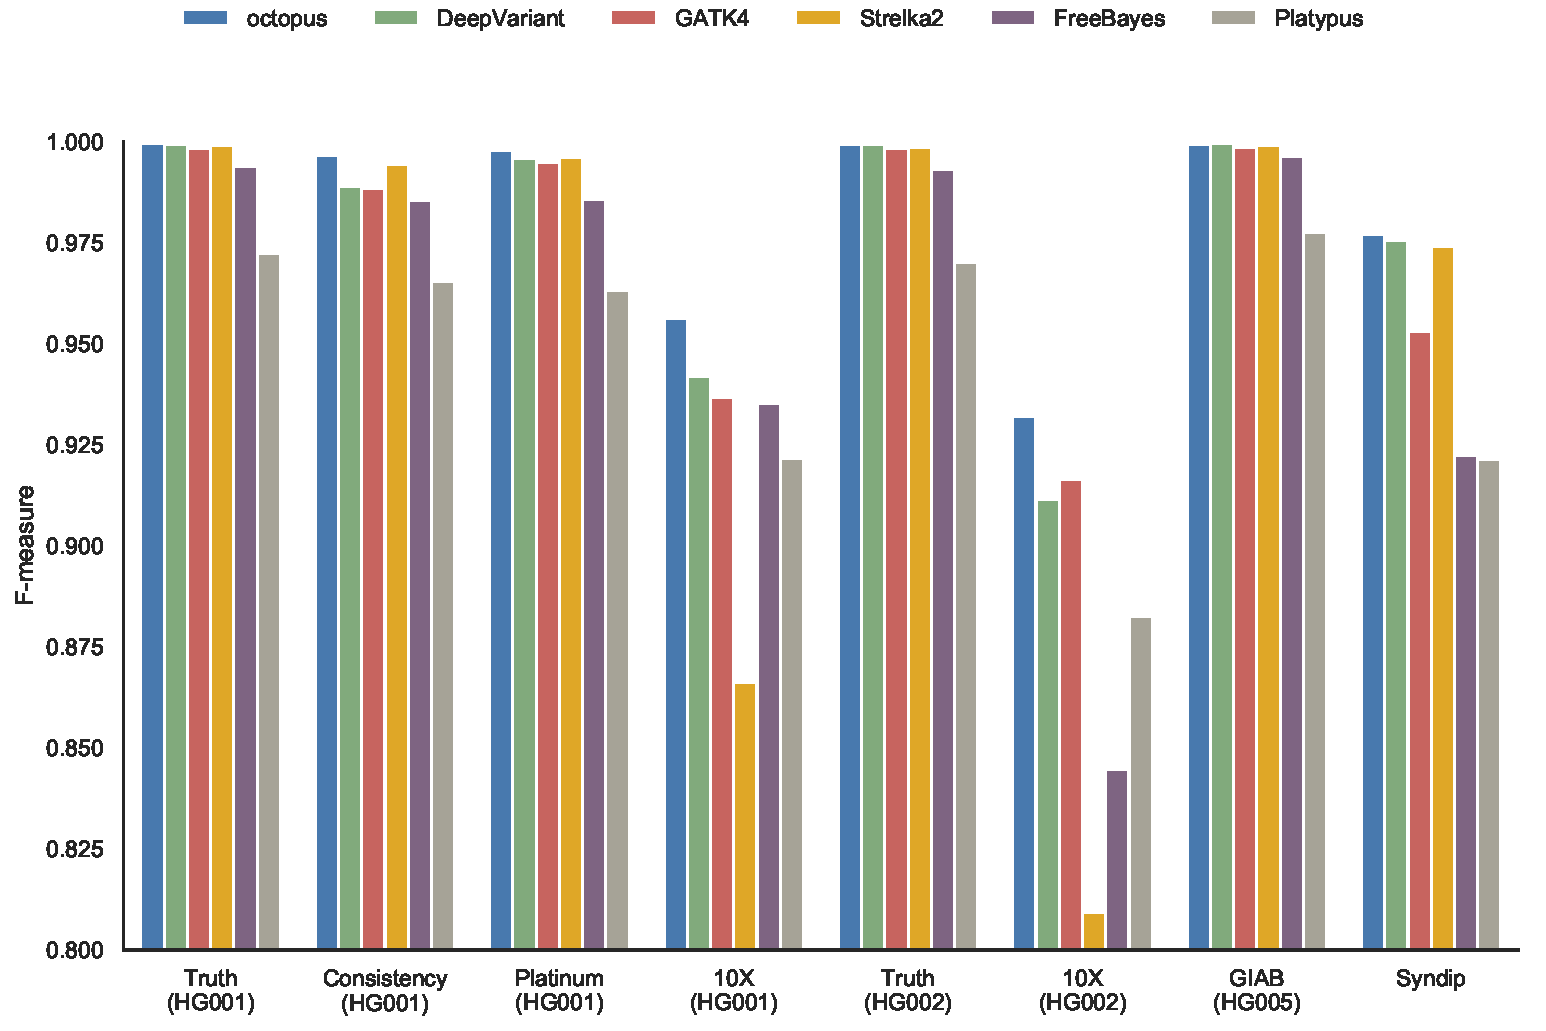
\includegraphics[width=\textwidth]{figures/F-Measures}
        \label{fig:germline:f-measure}
    \end{subfigure}
    \begin{subfigure}[b]{0.49\textwidth}
        \vspace{-0.5cm}
        \caption{}
        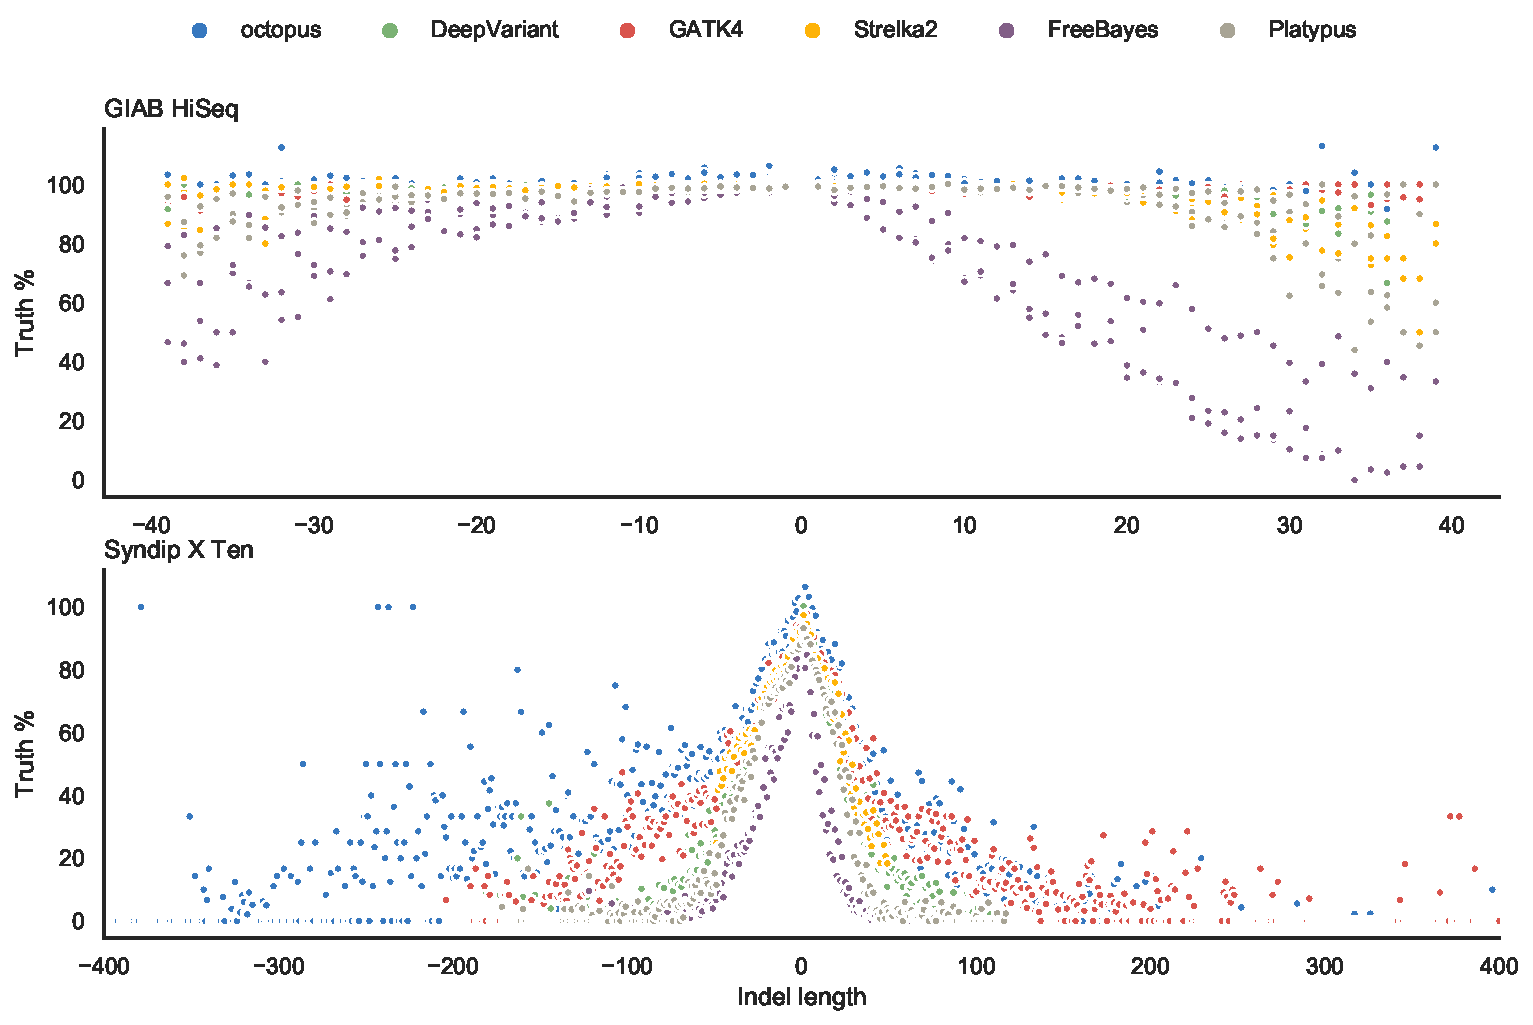
\includegraphics[width=\textwidth]{figures/indels}
        \label{fig:germline:indels}
    \end{subfigure}
    \vspace{-0.5cm}
    \caption{\textbf{Germline variant calling accuracy.} Comparison of Octopus with other methods on PrecisionFDA Truth Challenge HG001, GIAB 10X HG001, PrecisionFDA Consistency Challenge Garvan, Platinum Genomes HG001, PrecisionFDA Truth Challenge HG002, GIAB 10X HG002, GIAB HG005, and Syndip. The coverages of each dataset are approximately $50$x, $35$x, $40$x, $50$x, $50$x, $25$x, $50$x, and $40$x respectively. \protect\subref{fig:germline:precision-recall} Precision-recall curves showing accuracy on all test sets. Scoring metrics used to generate curves are RFQUAL, GQ, QUAL, GQX, GQ, and QUAL for Octopus, DeepVariant, GATK4, Strelka2, FreeBayes, and Platypus respectively. The dots show typical PASS thresholds: $3$ for Octopus, DeepVariant, and Strelka2; $20$ for GATK4, FreeBayes, and Platypus. \protect\subref{fig:germline:f-measure} F-Measures at PASS thresholds for each test set. \protect\subref{fig:germline:indels} Proportions of true indels called in comparison to the number in the truth set by indel length. Top: GIAB HiSeq tests (PrecisionFDA Truth Challenge HG001 \& HG002, and GIAB HG005). Bottom: Syndip}
    \label{fig:germline}
\end{figure*}

To establish germline calling accuracy we called variants in three well characterised Genome in a Bottle (GIAB) \cite{RN153} samples: HG001 (NA12878), HG002 (NA24385), and HG005 (NA24631). In addition, we called variants in the recently published Syndip sample that was compiled using an orthogonal approach to the GIAB validation sets, covers more of the genome, and has a larger range of indels \cite{RN605}. To account for different sequencing conditions we tested several HG001 and HG002 replicates, including two replicates sequenced using the 10X Genomics protocol. We downloaded publicly available BAM files for the two 10X tests (from GIAB) and the Syndip test (from the Broad institute), BWA-MEM \cite{RN539} was used to map all other data from raw FASTQ files. We compared Octopus to GATK4 \cite{RN598}, DeepVariant \cite{RN562}, Strelka2 \cite{RN604}, FreeBayes \cite{RN538}, and Platypus \cite{RN5}. GATK4, Strelka2, and Platypus were run in default configuration. We used the "x10" sequence error model for Octopus (see Methods) for the X Ten and X10 test, but was otherwise default settings were used. FreeBayes was run with default configuration but with genotype qualities requested. For DeepVariant we followed the whole genome case study on Github (r0.6). We used random forest filtering for Octopus trained on three independent NA12878 data sets (Supplementary), and default pass thresholds for DeepVariant and Strelka2. For Freebayes and Platypus we tried recommended hard filters, but we found that this deteriorated performance as quantified by the F measure (the harmonic mean of precision and recall), so we did not apply filters other than based on variant or genotype quality (QUAL and GQ). We found that using VQSR for GATK4 - as recommended by the best practise pipeline - degraded performance, so we only used QUAL for filtering GATK4 calls. All calls were evaluated with RTG tools vcfeval \cite{RN169}.

Octopus has the highest PASS F-Measure on all tests other than the HG005 test (Fig. \ref{fig:germline:f-measure}). Performance difference is marginal between Octopus, DeepVariant, and Strelka2 on the two Precision FDA Truth tests and GIAB HG005 test, all of which use data from GIAB sequenced on the Illumina HiSeq platform. Octopus substantially outperforms other callers on the two 10X Genomics tests that have lower coverage than the other tests in addition to considerably longer read pair insert sizes. It appears that Strelka2 is more sensitive to insert size than other callers. Octopus also has better performance on the Precision FDA Consistency and Syndip tests, both of which use data from the Illumina X Ten platform, but sequenced in different laboratories (Garvan institue and Broad institue, respectively). The X Ten platform has higher error rates than the HiSeq platform, suggesting that Octopus is more robust to high levels of noise than other tools. In addition, Octopus has near ideal receiver operating characteristic across all tests (Fig. \ref{fig:germline:precision-recall}), indicating that the probabilistic scoring criteria reports well calibrated probabilities.

We did not stratify our evaluation into SNVs and indels - as is common practice - because the true mutations that resulted in a haplotype are normally uncertain, and the representation used for the ground truth is biased towards the tools used to derivive it. For example, a sequence change of ...AAACCC... to ...AACCCC... could be explained either by a single SNV, or a pair of homopolymer indels. To demonstrate this, we compared the proportion of indels classified true positive with the number in the respective truth set for the two Precision FDA Truth tests and GIAB HG005 tests tests. We found that Octopus calls on average $1.5\%$ more true positive indels than the total number of indels in the truth set while other callers call $0.5\%$ or less (Fig. \ref{fig:germline:indels}), despite there being less than $0.1\%$ difference in overall sensitivity between Octopus and DeepVariant on these tests. This apparent contradiction must be due to Octopus calling indels in regions where other tools - and the truth sets - call SNVs that result in the same haplotype sequence. We observe similar behaviour in the Syndip test for indel lengths up to $5$bp (Fig. \ref{fig:germline:indels}). We also found that Octopus and GATK4 call considerably higher proportion of true large indels ($>50$bp) than other callers in the Syndip test.

\subsection*{Microinversion detection}

Octopus calls complex replacements when an observed sequence cannot be satisfactorily explained in terms of simple SNVs and indels. Microinversions are one such complex replacements that involve inversion of small ($3-200$bp) tracts of DNA. Microinversions have not been well studied, likely due to calling difficulties, but have been suggested to play a role in evolution and disease, including cancer \cite{RN561, RN560}. A method developed to identify microinversions reported an average of $3.8$ per individual in 1000G data \cite{RN560}. We identified a total of $152$ microinversions ranging from $3-98$bp in the four HG001 (NA12878) high-coverage replicates. $104$ of these were called in at least three of the replicates and $75$ were called in all four. Around half of the inversions called in all four NA12878 replicates were $20$bp or longer. We also found $103$ microinversions in the HG002 replicate, including a $3$bp inversion in the coding region of TTC6. $72$ of inversions detected in HG002 were also called in HG001. Although some of the microinversions called by Octopus have dnSNP entries, it appears that these have been identified as MNVs rather than as microinversions, and most also have decomposed entries (i.e. SNVs and indels). For example, a $3$bp microinversion called by Octopus in HG001 in a splice site of LIMD1, a possible tumour supressor, has a dbSNP entry (rs71615396). However, there are also entries for $3$ SNPs (rs62242177, rs62242178, rs63132361) composing the MNV. The SNV entries have frequency meta-information while the MNV does not.

\subsection*{\textit{De novo} mutations in parent-offspring trios}

Random germline \textit{de novo} mutations resulting from imperfections in the DNA replication process during meiosis provide the necessary genetic variation for evolution. They are also known to be causative of several Mendelian and polygenic diseases \cite{RN157, RN160, RN159}. Large scale characterisation of \textit{de novo} mutations in population studies reveals important insights into population structure and demographic history \cite{RN158}. The fidelity of the DNA replication process means the number of \textit{de novo} mutations expected per genome duplication event is estimated to be small, an average of 60 per meiosis in humans \cite{RN6}.

To assess \textit{de novo} calling performance, we ran Octopus using the trio calling model on whole genome data from a previously characterised WGS500 parent-offspring trio \cite{RN5}. We choose this data as the libraries were prepared directly from blood rather than cell lines. In addition to the $63$ \textit{de novo} mutations previously Sanger validated in this sample, we manually curated a further $33$ mutations by inspecting \textit{de novo} calls made by three or more callers, and all other \textit{de novo} calls from Octopus and GATK using realigned BAMs that both tools can generate (Supplementary Fig. ).

\begin{table}[hb!]
    \centering
    \caption{\textit{De novo} mutations called in WGS500 trio.}
    \label{table:denovo}
    \small
    \sffamily
    \resizebox{\linewidth}{!}{%
    \begin{tabular}{lcccccccc}
        \toprule
         & \textbf{TP SNVs} & \textbf{TP Indels} & \textbf{FN SNVs} & \textbf{FN Indels} & \textbf{FP} \\
        \midrule
        Octopus & 72 & 16 & 3 & 5 & 9 \\
        DeepVariant & 70 & 0 & 5 & 21 & 10306 \\
        Strelka2 & 75 & 5 & 0 & 16 & 1548 \\
        GATK4 & 46 & 4 & 29 & 17 & 90 \\
        FreeBayes & 73 & 5 & 2 & 16 & 339 \\
        Platypus & 72 & 4 & 3 & 17 & 163 \\
        \bottomrule
    \end{tabular}
    }
\end{table}

Only Octopus and GATK4 called a number of \textit{de novo} mutations within the currently accepted range (Table \ref{table:denovo}). Platypus and FreeBayes called approximately $2x$ and $3x$ more \textit{de novo} mutations than we would expect. In contrast, both DeepVariant and Strelka2 call considerably more \emph{de novo} mutations than expected, despite being the two most accurate germline callers after Octopus, demonstrating that strong germline calling performance does not necessarily imply high \textit{de novo} calling accuracy. Whilst we are confident the performance of the other callers could be improved with additional filtering, it is not always obvious how this is best achieved. For example, filtering DeepVariant calls by GQ resulted in almost complete loss of sensitivity before the number of false positives fell below $100$ (GQ: $46$, TP SNV: $9$, TP INDEL: $0$, FP: $90$). Similarly for Strelka2, we found that accuracy was highly sensitive to filtering by GQX: filtering by $\text{GQX} \ge 22$ resulted in $106$ false positives and $72$ true positives but filtering by $\text{GQX} \ge 23$ resulted in $41$ false positives and only $50$ true positives.

\subsection*{Synthetic tumours}

\begin{figure*}[ht!]
    \centering
\captionsetup[subfigure]{position=top,labelfont=bf,textfont=normalfont,singlelinecheck=off,justification=raggedright}
    \begin{subfigure}[b]{\textwidth}
        \vspace{-0.5cm}
        \caption{}
        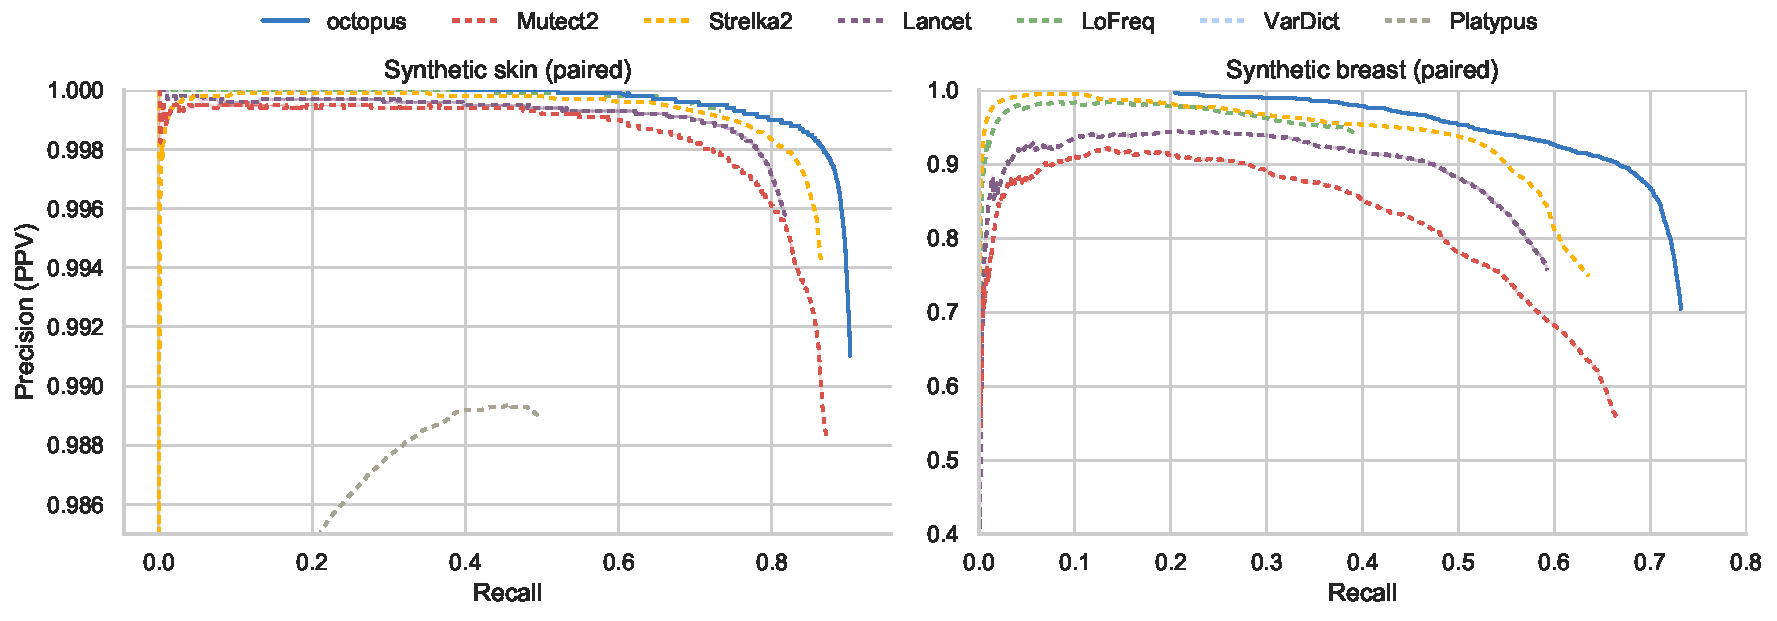
\includegraphics[width=\textwidth]{figures/somatic_precision_recall}
        \label{fig:somatic_pr}
    \end{subfigure}
    \begin{subfigure}[b]{\textwidth}
        \vspace{-1.0cm}
        \caption{}
        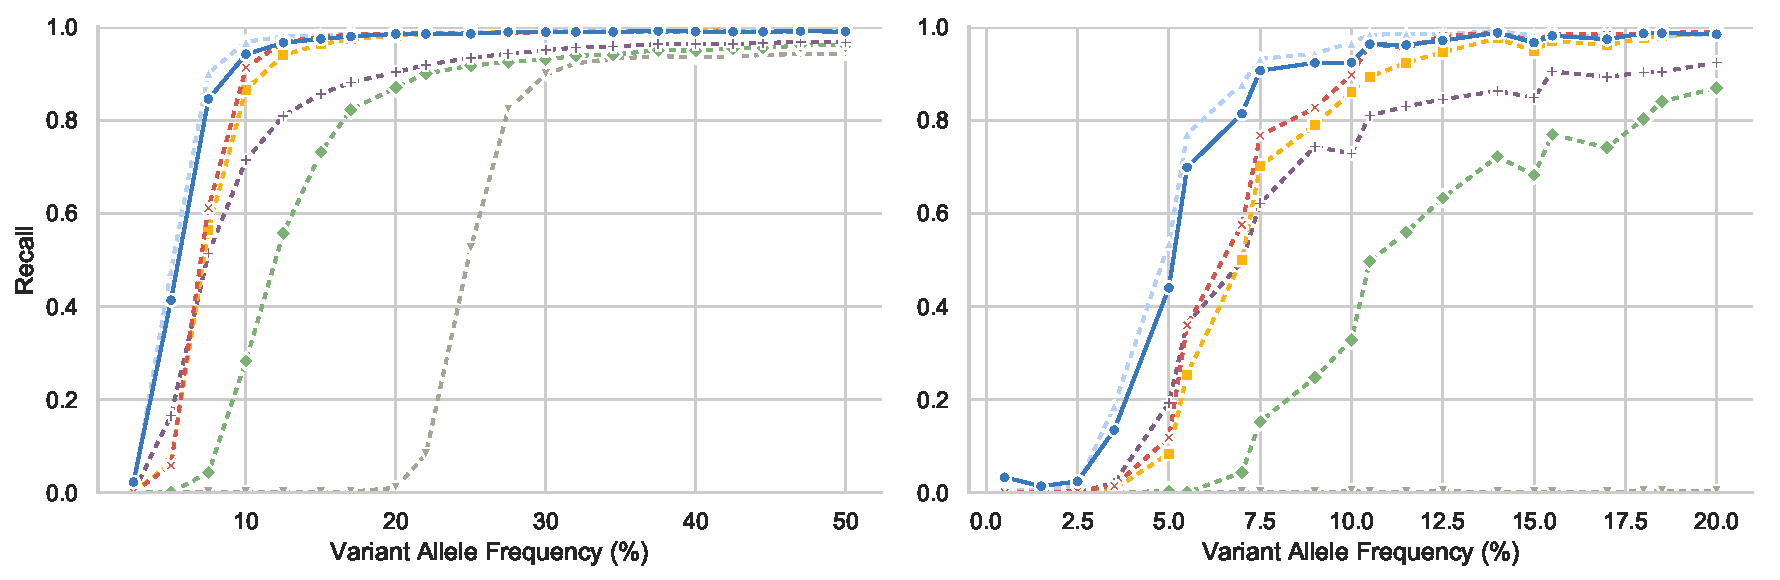
\includegraphics[width=\textwidth]{figures/somatic_vaf_recall}
        \label{fig:somatic_vaf_recall}
    \end{subfigure}
    \vspace{-1.0cm}
    \caption{\textbf{Paired somatic mutation calling accuracy.} \protect\subref{fig:somatic_pr} Precision/recall curves for paired-normal synthetic skin and breast tumours. Scoring metrics used to generate curves are RFQUAL, TLOD, and QSS for Octopus, Mutect2, and Strelka2 respectively and QUAL for Lancet, VarDict, and Platypus. VarDict is not visible as it is outside the axis limits due to low precision. Precisions on the two tests are substantially different as the skin set has almost $50$ times as many true mutations as the breast set. \protect\subref{fig:somatic_vaf_recall} Recalls for each Variant Allele Frequency (VAF) for paired skin and breast synthetic tumours. Points show true spike-in VAFs. The approximate depth for the synthetic skin and breast tumours were $60$x and $65$x, and $30$x and $35$x for their normal pairs, respectively.}
    \label{fig:syntumour}
\end{figure*}

Accurate benchmarking of somatic mutation calls is challenging because there is no gold standard reference to compare with, and different tumour types are known to have considerably different mutation profiles. Although calls may be manually validated to obtain an estimate of the false positive rate, it is not straightforward to estimate sensitivity as the ground truth remains uncertain. Although attempts have been made to accurately characterise somatic mutation profiles of real tumours by manual inspection \cite{RN155}, this process is limited by the power of existing tools, and is too time consuming to perform across a range of cancer types. An alternative strategy is to mix reads from unrelated individuals to create a synthetic tumour set \cite{RN142}. However, this approach is unlikely to yield tumours with realistic mutation profiles and haplotype structure. A third approach is to spike mutations directly into raw sequencing reads from healthy tissue, the approach taken by the ICGC-DREAM challenge \cite{RN147}.

We used an approach similar to that taken by the ICGC-DREAM challenge \cite{RN147}, with some modifications designed to ensure the synthetic tumours would have realistic mutation profiles and haplotype structures. The mutations we spiked in were taken from called somatic mutations from the PCAWG consortium, we used germline sequence data from a well-characterised sample (NA12878) for which high-quality germline haplotypes are available, and extended the tool BAMSurgeon to ensure mutations were spiked onto consistent germline haplotypes (\textbf{Methods}). We chose uniform spike-in frequencies rather than simulating sub-clonal structure, so that we could better access sensitivity at a range of variant allele frequencies.

We created two synthetic tumours for benchmarking using reads from GIABs $300$x NA12878 illumina data. The first was derived from skin cancer mutations using a mutation rate of $10^{-4}$ ($299,873$ mutations) and spike-in frequencies in the range $2.5$-$50\%$. The second derived from breast cancer mutations with mutation rate of $10^{-6}$ ($5,956$ mutations) and spike-in frequencies in the ranger $0.5$-$20\%$. The average depths were $60$x and $65$x respectively. Independent normal sets were created each synthetic tumour from remaining reads with average depths of $30$x and $35$x respectively.

\subsection*{Somatic mutations in paired tumour-normal samples}

We evaluated the accuracy of Octopus at calling somatic mutations in tumour-normal paired samples by calling variants in the skin and breast synthetic tumours. We trained Octopus's random forest classifier on chromosome X of the synthetic skin tumour data, which was removed from the test set. However, we found that Octopus was comparatively less reliant on filtering than other callers (Supplementary Fig. x). Calls were compared to MuTect2 \cite{RN142}, Strelka2 \cite{RN604}, LoFreq \cite{RN601}, Lancet \cite{RN600}, VarDict \cite{RN544}, and Platypus. We included Platypus, despite not being advertised as a somatic variant caller, to contrast germline and somatic callers, and because we are aware that germline callers (including Platypus) are sometimes integrated into somatic calling pipelines.

During the course of evaluation we discovered a small number (skin: $305$, breast: $209$) of calls not in the truth set but that appeared real mutations on manual inspection. This is not unsurprising since these data are derived from cell lines. To discount such cases we identified calls not in the truth set but called by at least $5$ of the $7$ callers tested, and removed these regions from evaluation. In addition, we found a small number of true mutations (skin: $2,766$, breast: $1$) that were incorrectly spiked in by BAMSurgeon, we therefore also ignored these regions during evaluation.

There is a clear trade-off between recall (sensitivity) and precision amongst callers. For example, Mutect2 and Strelka2 have almost identical F-Measures on the synthetic skin test ($0.9260$ and $0.9248$ respectively) despite Mutect2 showing better recall. VarDict has highest recall on both tests, but also has by far the worse precision. Lancet has moderate precision and recall. LoFreq has near perfect precision, but only Platypus has lower recall. Octopus has better recall than all callers other than VarDict, and only slightly worse precision than Strelka2. The number of false positive calls by each caller is similar in both tests suggesting that each caller has unique biases, although it is possible that some of these false positive calls are genuine cell-line artefacts.

Octopus shows considerably better precision-recall trade-off than the other callers tested, most notably at higher recalls. The default PASS threshold for Octopus is set reasonably low by default ($3$) to achieve high sensitivity, however, increasing the PASS threshold to $7$ (the default for Strelka2) reduces the number of false positives by over a third in both tests, while reducing the number of true positives by jusy $2.5\%$ and $6\%$ in the skin and breast tests, respectively.

Most of the differences in recall, particularly amongst the best performing tools (Octopus, Strelka2, Mutect2, Lancet), are due to low frequency mutations. Sensitivity for mutations below $2.5\%$ is poor for all callers ($0.01$ for Octopus and $0.002$ for Mutect2). At 60x sequencing depth, a $2.5\%$ VAF corresponds to an expectation of less than two observations. However, Octopus has considerably better sensitivity for mutations with VAFs between $4-10\%$ ($3$-$5$ expected observations at 60x) and has only slightly worse recall than VarDict, which represents an approximate upper-bound on sensitivity. Mutect2 has slightly better sensitivity at moderate VAFs ($12$-$20\%$). We note that Mutect2 was one of the callers used for PCAWG mutation calling, and on examination, some of these unique calls appeared to be calling artefacts.

\subsection*{Mutations in tumour-only samples}

Paired normal tissue samples are not always available when studying tumours from cancer patients, however, most somatic detection tools require a paired normal sample \cite{RN604, RN601, RN600}. We tested Octopus's tumour-only calling by calling variants in both synthetic tumours without providing the paired normals. We compared Octopus with a tool designed for calling unpaired tumour samples, Pisces \cite{RN602}.

\begin{figure}[ht!]
    \centering
\captionsetup[subfigure]{position=top,labelfont=bf,textfont=normalfont,singlelinecheck=off,justification=raggedright}
    \begin{subfigure}[b]{\linewidth}
        \vspace{-0.5cm}
        \caption{}
        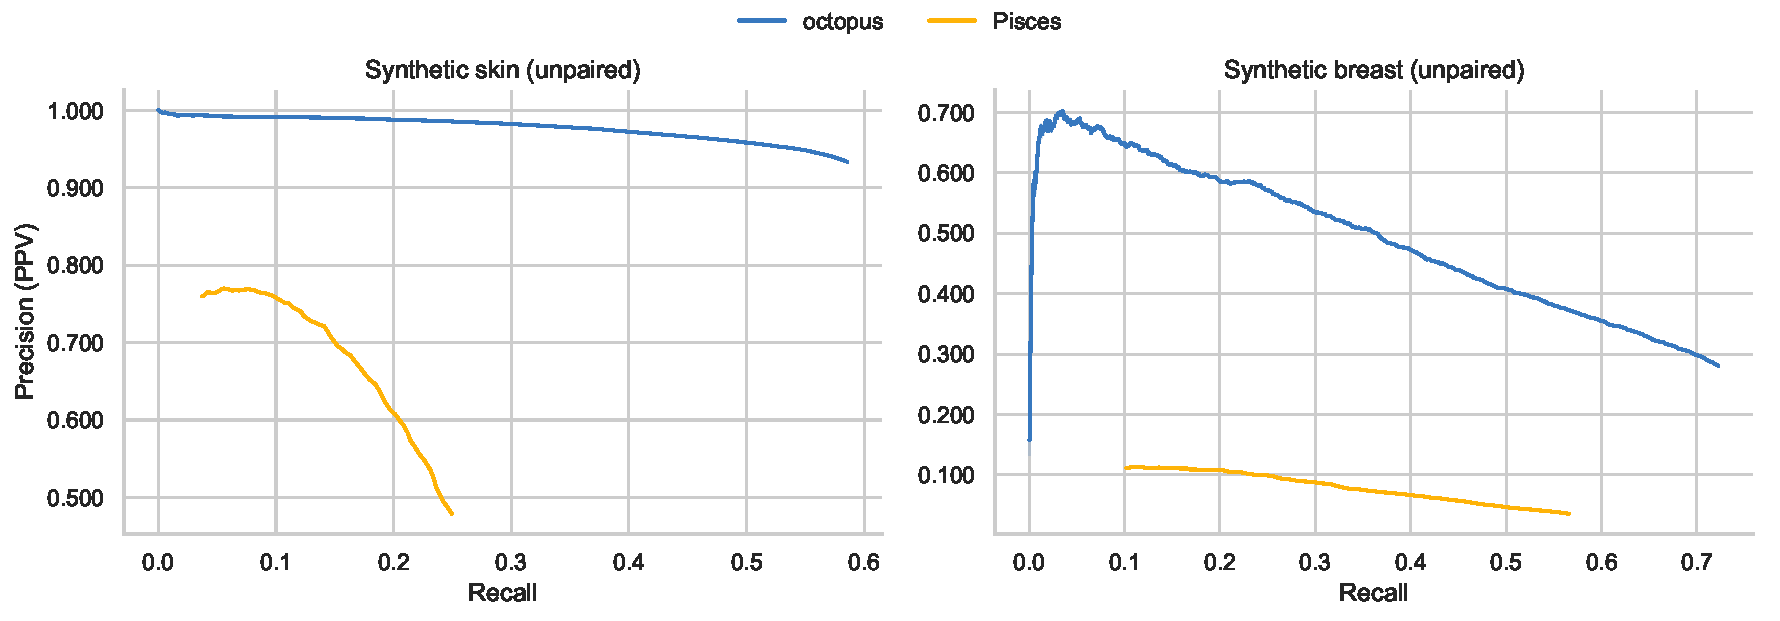
\includegraphics[width=\linewidth]{figures/tumour-only-precision-recalls}
        \label{fig:to-somatic_pr}
    \end{subfigure}
    \begin{subfigure}[b]{\linewidth}
        \vspace{-0.5cm}
        \caption{}
        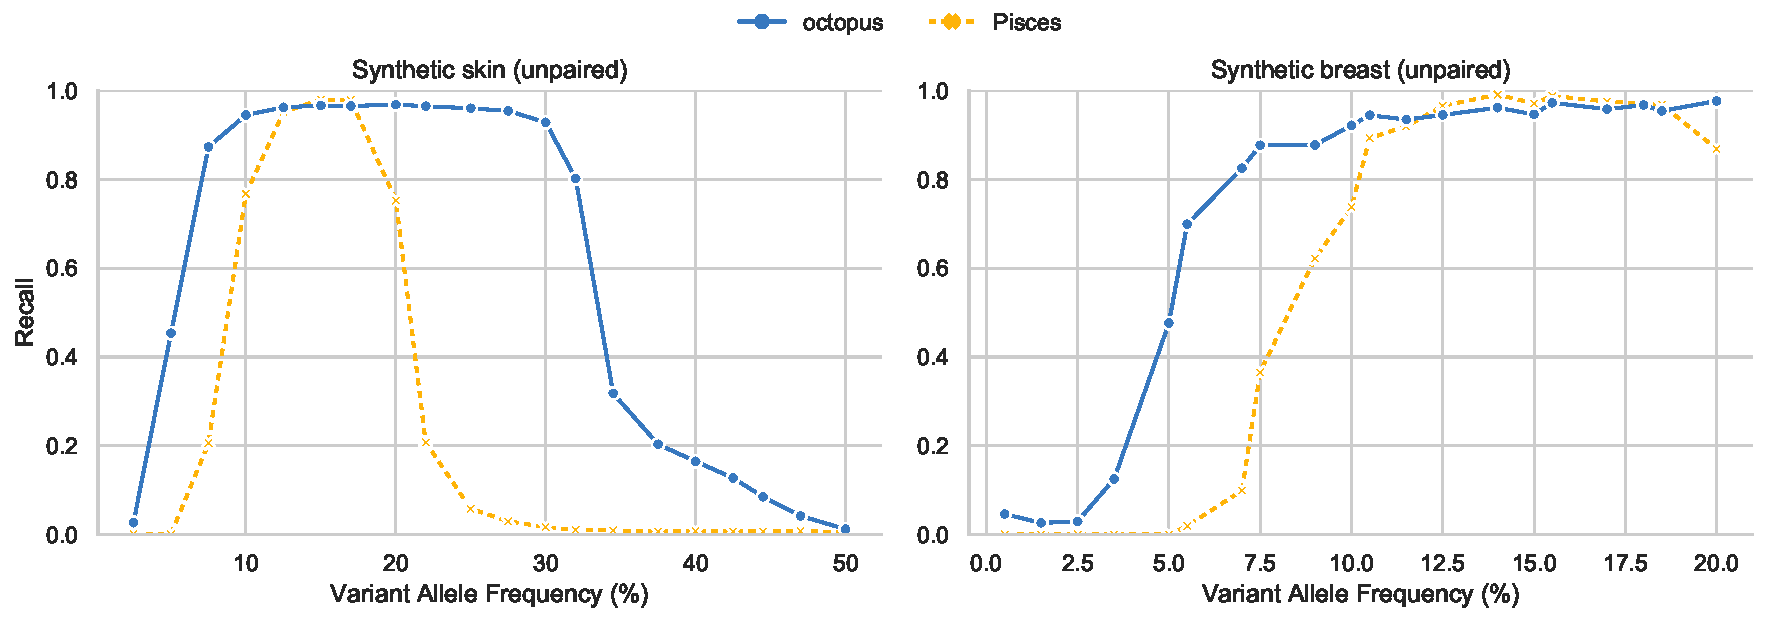
\includegraphics[width=\linewidth]{figures/tumour-only-vaf-recalls}
        \label{fig:to-somatic_vaf_recall}
    \end{subfigure}
    \vspace{-1.cm}
    \caption{\textbf{Tumour-only somatic mutation calling accuracy.} \protect\subref{fig:to-somatic_pr} Precision/recall curves for synthetic skin and breast tumours. \protect\subref{fig:to-somatic_vaf_recall} }
    \label{fig:syntumour-tumour-only}
\end{figure}

Unsurprisingly, Octopus' somatic calling accuracy is worse compared with the paired test, most notably the number of false positives is considerably higher on both tests. However, Octopus substantially outperforms Pisces both in terms of recall and precision (Fig. \ref{fig:to-somatic_pr}). Pisces calls $6.5x$ and $8.3x$ more false positive somatics as Octopus in the skin and breast tests respectively, yet Octopus calls $2.3x$ and $1.3x$ more true positives. The difference in sensitivity is primarily due to Octopus having higher sensitivity to a greater range of variant allele frequencies, in constrast to Pisces that is only sensitive to frequencies between $10$ and $20\%$ (Fig. \ref{fig:to-somatic_vaf_recall}).

A significant challenge with tumour-only calling, compared somatic calling with a paired normal sample, is correctly classification of variants as either somatic or germline. Both Octopus and Pisces are capable of calling and classifying both germline and somatic variants, and we observed that both callers misclassified a large number of true somatic mutations as germline polymorphisms in the skin test, which largely explains that observed drop-off in recall in the higher frequency range (Fig. \ref{fig:to-somatic_vaf_recall}). Octopus provides a measure of uncertainty in classification, which correlates with VAF (Supplementary Fig. z). Depending on the application, classification may or may not be important; it may suffice to know the variant is present even if the somatic status is uncertain. We therefore evaluated the performance of both callers on combined germline and somatic truth sets; ignoring somatic classification. We found that there was little difference in sensitivity between the callers, but a large difference in precision (Supplementary Fig. y). There were only marginally more false positive calls for Octopus on the combined test than the somatic-only test ($<1700$ in both tests), indicating that there are few germline calling errors, while Pisces calls over $17000$ additional false positives in both tests - an order of magnitude more than Octopus.

\subsection*{Phasing somatic mutations}

The germline haplotype that a somatic event mutates may be of high clinical relevance as it could determine loss of heterozygosity if there is already a loss-of-function mutation - germline or somatic - on the complementary germline haplotype. Furthermore, phasing information can be informative of tumour heterogeneity, which may have important clinical implications. To the best of our knowledge, no method is currently able to phase somatic mutations; either with germline polymorphisms or other somatic mutations.

Since we designed the synthetic tumours used to benchmark somatic mutation calling so that individual reads would respect haplotype structure (but not necessarily read pairs), we know the local phase of all somatic mutations. We investigated Octopus' ability to phase somatic mutations by evaluating how well Octopus was able to recover this phasing information in the skin synthetic tumour. We found that of the $257,930$ somatic mutations that Octopus calls, $57,217$ ($~22\%$) were phased with at least one heterozygous germline polymorphism. Furthermore, $9,834$ ($~4\%$) were phased with at least one other somatic mutation, and $2,848$ ($~1\%$) of these were also phased with a heterozygous germline polymorphism. We did not find any phasing errors (TODO: check!).

\section*{Discussion}

High-throughput sequencing is widely used throughout the genomics community, yet the most powerful variant calling methods are optimised for population data. Octopus should immediately be useful to the large number of researchers whom are currently using suboptimal variant calling stratagies. Our data indicate that Octopus is highly accurate on several important experimental designs, demonstrating the overall benefit of a unified haplotype-based approach. Although we did not include an evaluation of the polyclone calling model, intended for bacterial or viral sequencing protocols, we are confident that Octopus would perform well for this application, since the problem is similar to tumour-only calling without the additional challenge of somatic classification. 

We showed that Octopus is more robust to sequencing errors and depth than other callers on germline data, likely a result of the longer haplotypes that are used for inference. Although we only only considered one sequencing technology for the \textit{de novo} and somatic calling comparison, but we have every reason to believe that Octopus would be  

Our analysis of germline indels indicate that Octopus is able to call a wider ranger of indels than other methods. Octopus calls considerably more true short ($<15bp$) indels than other methods, and even more than is represented in the truth sets. One explanation for this is that existing methods systematically misclassify a large number of indels as SNVs in tandem repeat regions leading to underrepresentation in the truth sets. Although both representations result in the same haplotype sequence, such distinction could have important clinical consequences for some analyses, such as mutation signature decomposition \cite{RN86} or microsatellite instability testing. Moreover, around half of our manually curated \textit{de novo} calls occur in microsatellites. Such sites are known to have higher mutation rates than average but are almost always ignored in \textit{de novo} mutation studies because such regions are also difficult to precisely call. Our results indicate that Octopus is sufficiently specific for these mutations to be considered.

Microinversions have evaded comprehensive study because no commonly used short variant calling methods have been able to accurately call them. Our results provide evidence that these events are more common than previously thought, and possibly have functional consequence. In a follow up experiment, we found that Octopus called a considerable number of microinversions in Mycobacterium Tuberculosis isolates, almost all of which were found in Inverted Repeat (IR) motifs. This is also a feature of many of the microinversions that we found in human data. IR's are known to form cruciform extrusions causing genetic instability that results in high mutability, and have been shown to cause pathogenic mutations in cancer (cite). To our knowledge, microinversions have not previously been linked with IR's, but our data suggests this is the case. We suggest a simple mutational mechanism whereby DNA polymerase is temporarily dislodged and copies the complementary loop extrusion before reorienting on the forward strand.

Sensitivity to a wide range of variant allele frequencies is critical for accurate somatic mutation calling, however, our results suggest that existing somatic callers have poor sensitivity for low frequency variation at typical sequencing depths - unless a large number of false positives are accepted. Octopus shows near optimal sensitivity across all variant allele frequencies while remaining highly specific. Octopus is likely more able to discern noise from real variation as a result of longer haplotypes, better error modelling, and more realistic mutation priors.

Our analysis of somatic mutation phasing indicate that Octopus could be used to detect cases of biallelic loss-of-function mutations, and possibly provide information on sub-clonal architecture, beyond the information already provided by variant allele frequency inference. 

Finally, Octopus has a number of usability advantages over existing tools: Reads do not require pre-processing as this is done internally, simplifying workflows and eliminating the need to copy BAM files. As an illustrative example, we needed over $20$ commands to call \textit{de novo} mutations with GATK4 compared with one for Octopus. Furthermore, multithreading is built-in, and disk access is optimised for few long accesses rather than many short accesses, which is generally better for disk health. Octopus is capable of producing realigned 'evidence' BAMs, including for somatically mutated haplotypes. We hope that clinicians in particular will find this feature useful for aiding call validation and interpretation.

As new experimental designs emerge, the flexibility of our method should allow us to rapidly incorporate new genotype models that take full advantage of the information provided by individual technologies. Single cell sequencing is just one example that is on our radar.

% Octopus uses the same probabilistic model for paired and unpaired tumour calling; only the prior distribution for the normal sample changes (Online methods). The behaviour of the model without a normal sample is demonstrative of the Bayesian approach. At low VAFs ($<10\%$), recalls are very similar to the paired tests. However, at moderate VAFs ($10-30\%$) recalls level off for unpaired but continue to increase for paired. As VAF increases there is more evidence that a mutation exists. Without a normal sample there is usually, but not always, increasing evidence that the mutation is a \emph{germline} variant. There are two ways increasing VAF could favour the somatic hypothesis over germline Interestingly, between these moderate VAFs the evidence for these competing hypothesis balances almost exactly. Beyond these frequencies the model prefers the germline explanation. Although Octopus classifies all calls as somatic or germline, it also reports a measure of confidence in this classification which could help prioritise called germline variants that are incorrectly classified.

\bibliographystyle{plos2009}
\bibliography{Octopus-paper}

\section*{Methods}\small

\subsection*{Read pre-processing}

Input reads are scanned in random sub-regions of the input region set to estimate basic statistics such as average depth and read lengths. These statistics are used to determine sub-regions of the input regions to buffer input reads, so that the memory occupied by read data is below a user-defined limit. If multiple threads are requested then the buffer limit is shared evenly between threads. Input read files can contain multiple samples, but must have associated read group information.\\

\emph{Transformations.} Read transformations adjust the data contained in a read observation without removing the read. Most of the transformations recalibrate base qualities in certain ways. The current list of available read transformations is:

\begin{itemize}
\item Cap the maximum base quality of all bases
\item Set base qualities of putative adapter bases to zero
\item Sets base qualities of bases overlapped by multiple templates from the same read segmenet to zero on all but one of the template
\item Mask low quality tails
\item Mask low quality soft clipped bases
\end{itemize}

\emph{Filtering.} Read filters remove reads that are likely problematic and cannot be transformed into something useful. Read filtering is applied \emph{after} read transformations. Reads are filtered if \emph{any} of the given filtering predicates fails. The current possible read filter predicates are:

\begin{itemize}
\item Malformed CIGAR
\item Unmapped
\item Low mapping quality (user defined)
\item High fraction of low quality bases (user defined)
\item Marked QC fails
\item Short or long (user defined)
\item Marked duplicates
\item Duplicates identified by Octopus
\item Secondary alignments
\item Supplementary alignments
\item Reads with likely adaptor contamination
\end{itemize}

\emph{Downsampling.} Read downsampling removes reads to satisfy user specified depth criteria. Sample read sets are downsampled independently. First, regions that have depth above a certain threshold are detected. Using existing mapping formation, we calculate how many reads such be removed for each position. Reads in  are then removed iteratively by first selecting a position to downsample with probability proportional to the required depth reduction at positions, and then selecting a read overlapping that position with uniform probability.

\subsection*{Candidate allele discovery}

Candidate alleles are generated jointly for all samples by taking the union of candidates generated from a set of orthogonal methods (\emph{generators}). Users can choose which generators to use to optimise accuracy and runtime. The read-backed generators can be tuned to increase sensitivity for low-frequency variation.\\

\emph{Pileups.} Uses the read mapping and alignment information present in the input BAM files and proposes candidates bases on mismatches present in these alignments. Alleles are only proposed if the observation of a particular satisfies some inclusion predicate, which primarily depends on the observation frequency; observed base qualities; and observation read strands.\\

\emph{Local reassembly.} Discards read alignment information (but keeps mapping location) and builds a kmer based assembly graph (i.e. \emph{de Bruijn} graph) at regions considered likely to contain variation. Once the graph is constructed, paths with low observation kmer counts and cycles are pruned. Candidate alleles are extracted by enumerating the highest scoring non-reference bubbles, where the score is determined by the sum of the kmer counts, weighted by strand bias. The non-reference path of the bubble is aligned to the reference to form candidate alleles. Complex variation such as microinversions are found by inspecting bubbles.\\

\emph{Repeat realignment.} Identifies common patterns of misalignments in tandem repeat regions that results in runs of regularly spaced SNV mismatches and manually proposes indel candidates.\\

\emph{Input VCF.} Takes a set of user specified VCFs and extracts all alleles present in the region to be called. Filtering dependent on the QUAL of each site is optional.

\subsection*{Candidate haplotype generation}

\emph{Construction.} Haplotypes are exhaustively constructed from all candidate allele combinations. This approach differs from other approaches which construct haplotypes directly from read observations \cite{RN141, RN538}. The primary advantage of our method is that haplotypes with no direct read support are proposed, so the length of haplotypes is not limited by read length. However, since the number of haplotypes is exponential in the number of alleles this approach is usually only feasible for very short haplotypes. To allow construction of long haplotypes, we developed a graph-based data structure, termed \emph{haplotype-tree}, where tree-nodes are alleles, and branches are unique haplotypes. The key property of the haplotype-tree is that individual branches (haplotypes) can be removed or extended, which allows us to limit the haplotypes in the tree to only the most likely ones given the current state of knowledge.\\

\emph{Deduplication.} It is possible that duplicate haplotypes (i.e. identical sequence) exist in the haplotype tree since candidate alleles are exhaustively combined. Duplicate haplotypes will have identical likelihoods as the probability of generating a read from a haplotype is only a function of the sequence itself. However, duplicate haplotypes may not have equal posterior probability as the prior probability of a haplotype segregating depends on the alleles which compose the haplotypes. Since the posterior of duplicate haplotypes is only dependent on the prior we just keep the duplicate with the greatest prior probability.\\

\emph{Filtering.} There are two haplotype filtering stages; prior and post to genotype inference. The latter is always preferable as it is possible to deduce a marginal posterior probability for each haplotype segregating in the samples, which contains all possible information. In constrast to the former which must use approximation. However, for efficiency reasons, it may sometimes necessary to reduce the number of haplotypes considered by the genotype model. While there is no silver bullet strategy, we have found likelihood based approaches are most effective. In particular, we reduce the number of haplotypes to a user defined threshold by ranking haplotypes by the number of reads assigned to each haplotype calculated by maximum likelihood.

\subsection*{Haplotype likelihood calculation}

\emph{Remapping.} The first step of the likelihood calculation is to remap reads to candidate haplotypes. This is required because the likelihood model requires that reads already be reasonably well placed, and the mapping position provided by the read mapper may not be accurate with respect to certain haplotypes (e.g. when indels are present).

We use a simple \emph{k-mer} based mapper to find putative mapping locations. Briefly, the k-mer ($k$ is hard coded) starting at each read and haplotype base are calculated. For each k-mer in the read we then see if that k-mer exists in the haplotype, and if it does, we calculate where in the haplotype the read should start assuming perfect alignment between the read and haplotype up until the k-mer (i.e. offset by the k-mer position in the read) and increment a 'hit' count at that position. After doing this for all k-mers in the read we look for positions in the haplotype that have high hit counts and emit these as putative mapping positions.\\

\emph{Error models.} Sequencing error models parameterise the likelihood HMM with indel gap open, gap extension, and optionally, SNV mismatch caps. The current implementation uses a constant gap extension penalty. The penalties are set according to local repeat context, up to some maximum repeat period (default 3 - trinucleotide repeats). There are currently two sequence error models: the default, which is intended for typical Illumina HiSeq quality data, and one intended for sequencing machines with higher error rates, such as the Illumina X Ten platform. We did not use any automated inference procedure to arrive at the parameters for these two models; we set them to reasonable values based on experience and observation.\\

\emph{pHMM.} Haplotype likelihoods are calculated using a pair hidden Markov Model (pHMM). The pHMM likelihood method computes the approximate Viterbi probability of the read given the haplotype. We use the Viterbi probability rather than the forward probability since the Viterbi probability is considerably cheaper to compute in log space, and in practice the difference between using the two probabilities is small. The simplest pHMM implementation has positional gap open penalties which are a parameter to the model. There is a second version of the pHMM that also has so-called 'SNV' mismatch caps. This a vector of nucleotides and maximum base mismatch penalties, one for each position in the haplotype sequence, that limit the penalty of a mismatch aligned to that position where the mismatching read base is the nucleotide indicated in the provided vector. The intention of this is to model a common error mode in sequencing data in repetitive regions, especially homopolymers, where a single base on the edge of the repeat 'falls over' to the leading base of the repeat.

The pHMM is a critical bottleneck in Octopus and is therefore uses a highly optimised banded SIMD implementation. Being banded, the likelihood calculation only explores parts of alignment space that results in indels less than the band size (currently 8). For short Illumina quality reads, this limitation is almost never an issue as indel \emph{errors} greater than this are extremely rare. For longer, noisier reads, the band size would need to be increased. Since the band size is just the width of the SIMD register used by the implementation (currently SSE2), to achieve a larger band size we would need to modify the code to use SIMD instructions that support larger register sizes (e.g. AVX2).\\

\emph{Inactive flank scoring.} An important feature of our pHMM likelihood calculation is dubbed \emph{inactive flank score discounting}. To understand this calculation, it is important to remember that candidate haplotypes in Octopus are constructed from a set of candidate alleles. However, it may be the cases that the true haplotype that a given read originates from is only partially formed in the set of candidate haplotypes. This can either be the case if the haplotype generator is yet to active an allele (i.e. the true allele is to the right of the current active set), or that the allele was deactivated and now lies to the left of the current active set. If this is the case, then the likelihood for a true haplotype could be lower than a false one only because the false one better support a true haplotype that has yet to be considered. This, in short, is the 'windowing' problem that all haplotype methods must address. Octopus' solution to the windowing problem is to only commit to calling candidate alleles once there is reasonable confidence that the reads supporting the alleles have had likelihoods evaluated on \emph{all} the true alleles they support. However, the problem still remains that we must evaluate the likelihood function with a haplotype that is correct in the active region, but false outside this region (sequences outside the active region are always padded with reference). To overcome this, we would like to 'discount' any reductions to the likelihood that arise from mismatches outside the active region. We do this by retracing the Viterbi path and subtract terms from the log likelihood that are due to mismatches outside the active region. This feature can be disabled by the user.\\

\emph{Mapping qualities.} Mapping quality is an important mapping statistics that reflects the trustworthiness of a reads mapping location. Formally, it has been defined as the probability the read alignment is wrong. In Octopus, we are not so concerned with the \emph{alignment} of a read since all reads are realigned internally. However, if the read is incorrectly placed, to the degree that the remapping step cannot place the read correctly, then the read is not informative of the true haplotype and should not be used. 

\begin{align*}
	p(r | h) &= p(r | h, \text{mapped})p(\text{mapped}) \\
              & \quad + p(r | h, \text{missmapped})p(\text{missmapped})\\
	         &= p(r | h, \text{mapped})q + p(r | h, \text{missmapped})(1 - q)
\end{align*}

Where $q = 1 - 10^{\frac{-\text{MQ}(r)}{10}}$. $p(r | h, \text{mapped})$ is then simply the likelihood from the pHMM. $p(r | h, \text{missmapped})$ is a more interesting quantity. If the read is unmapped, then it originated from some other sequence not localised to the reference region used to construct the haplotype under consideration. There are three possibilities we must consider: i) The read originates from a region of the genome not included in the reference build. ii) The read originates from another genome (i.e. contamination). iii) The mapper made an error; the true mapping position in the reference build. TODO

\subsection*{Mutation models}

\emph{Indel mutation model.} Local gap open and extension probabilities are modelled for germline, \textit{de novo}, and somatic mutations with a single indel mutation model. The model takes as input a basic rate parameter which is scaled according to the local repeat composition of the sequence using the model in Montgomery et al \cite{RN577}. Gap extension probabilities are assigned bases on repeat composition and existing repeat length. The main behaviour of the extension model is to assign high probability to extensions of incomplete repeat periods as indels in tandem repeats almost always occur in whole periods.\\

\emph{Coalescent mutation model.} The coalescent mutation model assigns probabilities to sets of haplotypes assumed to be sampled randomly from an idealised population.

There are two parameters to the model: $\theta_1$ is the SNV heterozygosity, $\theta_2$ is the indel heterozygosity. $\theta_1$ is set depending on user input. $\theta_2$ is set according the the indel mutation model given the reference sequence and a user input indel heterozygosity value. The maximum indel gap open heterozygosity is used.

For a given set of haplotypes ${\boldsymbol{h} = \{h_1, \dots, h_m\}}$ we first calculate two quantities: $k_1$ is the number of unique segregating SNV sites observed in $\boldsymbol{h}$ and $k_2$ is the number of unique segregating indel sites observed in $\boldsymbol{h}$. Both values are calculated by comparing the alleles composing haplotypes to the reference haplotype. 

Probability is then assigned to $\boldsymbol{h}$ using the forumula:

\begin{equation*}
    p(\boldsymbol{h}) = \binom{\theta_1}{\theta_1 + \theta_2}^{k_1} \binom{\theta_2}{\theta_1 + \theta_2}^{k_2} \binom{k_1 + k_2}{k_1} p_{\theta = \theta_1 + \theta_2} (k_1 + k_2)
\end{equation*}

Where $p_\theta(S = k)\sum_{i=2}^n (-1)^i \binom{n - 1}{i - 1} \binom{i - 1}{\theta + i - 1} \binom{\theta}{\theta + i - 1}^k$. Which is an extension of formula $4.3$ found in John Wakeley's Coalescent theory.

We note a limitation of this model is that only a single indel heterozygosity value is used for all positions in the observed haplotypes. While this assumption is unrealistic, it turns out not to be particularly detrimental since the most important aspect of the model is to assign high likelihood to indels in repeat regions. The likelihood of proposing some other spurious indel in a region outside the repeat region is small given the haplotype lengths normally considered. We could look to address this issue in the future, particularly if the algorithm is updated to handle long-read data.\\

\emph{De novo and somatic mutation models.} The \textit{de novo} mutation model is intended assign probabilities to \textit{de novo} mutation occurring on a single haplotype during a single DNA replication. Formally, given an known haplotype $h_1$, the model assigns probabilities $p(h_2 | h_1)$ where $h_2$ is another haplotype (note that we can have $h_1$ = $h_2$). The model assigns probabilities according to the indel mutation model and a SNV mutation rate that are parameters to the model. The somatic mutation model assigns probabilities to somatic mutations occurring on a single haplotype over some time period and is identical to the \textit{de novo} mutation model.

\subsection*{Genotype prior models}

Genotype prior models are used to assign prior probability to arrangements of genotypes. There are two types of genotype prior models: single and joint. Single genotype prior models assign probability to single genotypes, $p(g | \mathcal{M})$, joint genotype prior models assign probability to a \emph{combination} of genotypes, $p(\boldsymbol{g} | \mathcal{M})$. In some cases, such as the Coalescent genotype prior model, the former is simply a particular instance of the first, although it may have a separate implementation for efficiency. We report the unnormalised versions of each genotype prior model since normalisation is trivial, and is always performed as part of the genotype posterior model in any case.\\

\emph{Uniform genotype prior model.} The uniform genotype prior model, $\mathcal{M}_{uni}$, is the simplest genotype prior model. We have:

\begin{equation*}
    p(g | \mathcal{M}_{uni}) = 1 \quad p(\boldsymbol{g} | \mathcal{M}_{uni}) = 1
\end{equation*}

for the single case, and for the joint case, respectively. \\

\emph{HWE genotype prior model.} The Hardy-Weinberg Equilibrium (HWE) genotype prior model, $\mathcal{M}_{hwe}$, assigns probability to genotypes assuming HWE. The model is paramertised by a set of known haplotypes $\boldsymbol{h} = \{h_1, \dots, h_m\}$, and their frequencies, $f_i$ (for $i = 1 to m$). The haplotype frequencies may be set explicitly, or calculated with empirical Bayes. We recall the the HWE is simply a multinomial distribution:

\begin{equation*}
    p(g | \mathcal{M}_{hwe}) = \binom{|g|}{o_1(g), \dots, o_m(g)} \prod_{i=1}^m f_i^{o_i(g)}
\end{equation*}

where $o_i(g)$ is the number of times haplotype $i$ occurs in genotype $g$.\\

\emph{Coalescent-HWE genotype prior model.} The coalescent-HWE genotype prior model, $\mathcal{M}_{coal-hwe}$, is suitable for modelling germline genotypes; it is the default germline prior model for all calling models. There are two components to this model: a \emph{segregation} model, that assigns probability to the pattern of observed alleles in the genotype(s); and a \emph{frequency} model that assigns probability to the frequency each haplotype is observed. In particular, the segregation model is just the coalescent mutation model and the frequency model is a Hardy-Weinberg model parameterised with empirical Bayes. We then have:

\begin{equation*}
    p(\boldsymbol{g} | \mathcal{M}_{coal-hwe}) = p(\boldsymbol{g} | \mathcal{M}_{coal}) p(\boldsymbol{g} | \mathcal{M}_{hwe})
\end{equation*}

for the joint case. The individual case can be optimised to

\begin{equation*}
    p(g | \mathcal{M}_{coal-hwe}) = p(g | \mathcal{M}_{coal})
\end{equation*}

when $|g| \le 2$ (i.e. the sample is haploid or diploid) since $p(g | \mathcal{M}_{hwe})$ is then constant.\\

\emph{Trio genotype prior model.} The trio genotype prior model, $\mathcal{M}_{trio}$, assigns probabilities to triplets of genotypes that originate from parent-offspring trios. This model encapsulates two elements of uncertainty: inheritance patterns and parental haplotype modification due \textit{de novo} mutations. The model uses Coalescent-HWE genotype prior model or uniform prior model to assign probability to parental genotypes and the \emph{de novo} mutation model to model modifications to parental haplotypes. Let $g_m$, $g_p$, $g_o$ be the maternal, paternal, and offspring genotypes, respectively. This model then calculates $p(g_m, g_p, g_o | \mathcal{M}_{trio})$.

\begin{equation*}
    p(g_o, g_m, g_p | \mathcal{M}_{trio}) = p(g_m, g_p | \mathcal{M}_{g}) p(g_o | g_m, g_p, \mathcal{M}_{denovo})
\end{equation*}

The form of the latter term $p(g_o | g_m, g_p, \mathcal{M}_{denovo})$ is dependent on meiosis and fertilisation in the species under consideration. We only consider the mammalian case here.

Writing $\mathcal{M}_{d} \equiv \mathcal{M}_{denovo}$ for brevity. In the autosomal (i.e. all diploid) case, we have

\begin{align*}
    p(g_o | g_m, g_p, \mathcal{M}_{d}) &= \frac{1}{2} p(g_{o0} | g_m, \mathcal{M}_{d})p(g_{o1} | g_p, \mathcal{M}_{d}) \\ &+ \frac{1}{2} p(g_{o1} | g_m, \mathcal{M}_{d}) p(g_{o0} |g_p, \mathcal{M}_{d})
\end{align*}

reflecting the uncertainty in parental origin of the offspring haplotypes, and where

\begin{equation*}
p(g_{oi} |g_s, \mathcal{M}_{d}) = \frac{1}{2} p(g_{oi} | g_{s0}, \mathcal{M}_{d}) + \frac{1}{2} p(g_{oi} | g_{s1}, \mathcal{M}_{d})
\end{equation*}

models uncertainty in which parental haplotype is inherited. $p(g_{oi} | g_{sj}, \mathcal{M}_{d})$ is the probability the haplotype $g_{oi}$ is inherited by the child given that the haplotype $g_{sj}$ is the one provided by the parent $s$ for fertilisation; it models \textit{de novo} mutations.

For the female offspring X chromosome case we have the same form for $p(g_o | g_m, g_p, \mathcal{M}_{d})$ as the autosomal case, but

\begin{equation*}
p(g_{oi} | g_p, \mathcal{M}_{d}) = p(g_{oi} | g_{s0}, \mathcal{M}_{d})
\end{equation*}

For the male offspring X chromosome case we have

\begin{equation*}
 p(g_o | g_m, g_p, \mathcal{M}_{d}) = p(g_{o0} | g_m, \mathcal{M}_{d})
\end{equation*}

Finally, in the male offspring Y chromosome case we simply have

\begin{equation*}
 p(g_o | g_m, g_p, \mathcal{M}_{d}) = p(g_{o0} | g_{p0}, \mathcal{M}_{d})
\end{equation*}

\emph{Cancer genotype prior model.} The cancer genotype prior model, $\mathcal{M}_{cancer}$, is used to assign probability to \emph{cancer genotypes}. A cancer genotype is a pair of regular genotypes, $g_{cancer} = (g_{germ}, g_{som})$, where $g_{germ}$ is the germline and $g_{som}$ is acquired somatically. The model must explain both the germline and the somatic genotypes. No assumptions of either germline or somatic genotype ploidy are made.

The model $\mathcal{M}_{cancer}$ is the composition of two independent models: a germline prior model, $\mathcal{M}_{germ}$ (e.g. the coalescent-HWE model); and a \emph{conditional somatic model}, $\mathcal{M}_{som}$. We then have (omitting models for brevity)

\begin{equation*}
 p(g_{cancer} | \mathcal{M}_{cancer}) = p(g_{germ}) p(g_{som} | g_{germ})
\end{equation*}

The second term $p(g_{som} | g_{germ}, \mathcal{M}_{som})$ models the \emph{pattern} of somatic haplotypes. In the simplest case when $|g_{som}| = 1$ (i.e. there is a single somatic haplotype) then we just have

\begin{equation*}
	p(g_{som} | g_{germ}) = \frac{1}{|g_{germ}|} \sum_{i = 1}^{|g_{germ}|} p(g_{som,0} | g_{germ, i})
\end{equation*}

where $p(g_{som,0} | g_{germ, i}, \mathcal{M}_{som})$ is just the probability of observing the somatic haplotype given the germline haplotype $g_{germ, i}$ suffers some mutational event (which in theory could lead to the same sequence); it is just the somatic mutation model.

More interesting is when $|g_{som}| > 1$ (i.e. there are more than one somatic haplotypes). In principle, we must consider that any of the somatic haplotypes could have originated from either the germline \emph{or any other somatic haplotype}; we should consider possible tumour phylogenies. We have not implemented such a model in Octopus; we assume independence between somatic haplotypes:

\begin{equation*}
p(g_{som} | g_{germ}) = \prod_{j = 1}^{|g_{som}|} p(g_{som,j} | g_{germ})
\end{equation*}

\subsection*{Genotype posterior models}

\begin{figure*}[ht]
    \centering
    \begin{subfigure}[b]{0.3\textwidth}
        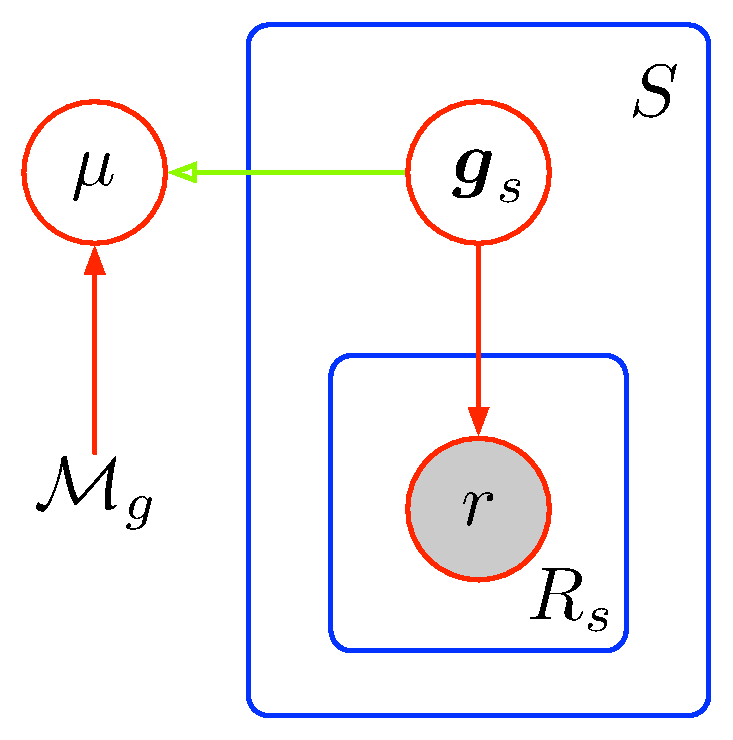
\includegraphics[width=\textwidth]{figures/population_model}
        \caption{}
        \label{fig:pop}
    \end{subfigure}
    \hfill
    \begin{subfigure}[b]{0.3\textwidth}
        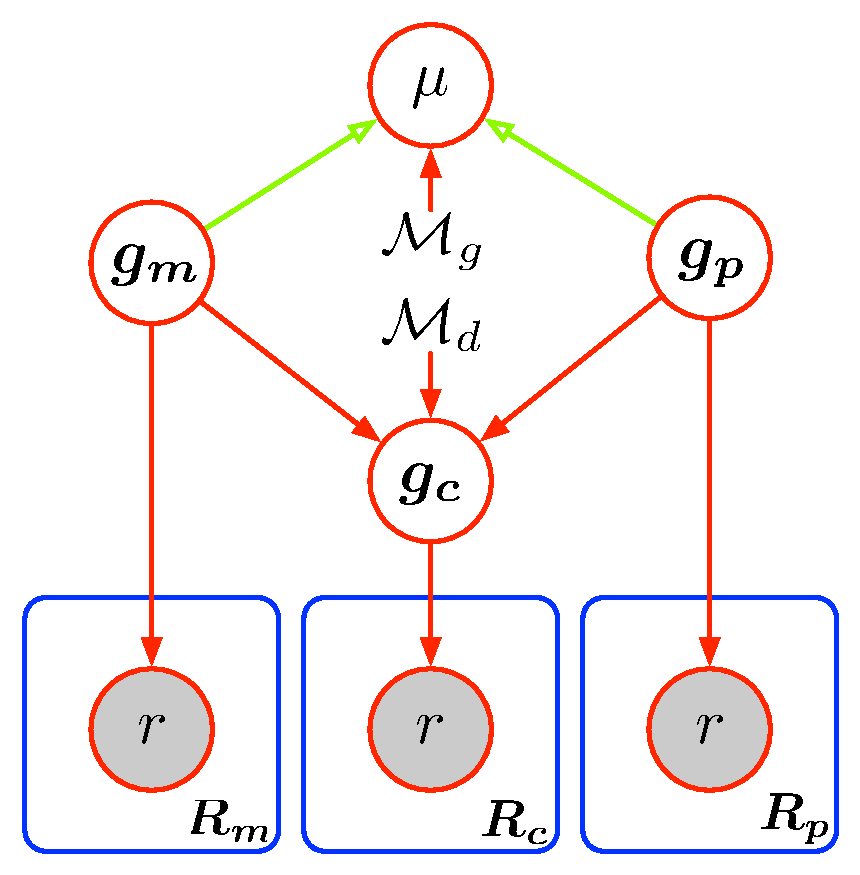
\includegraphics[width=\textwidth]{figures/trio_model}
        \caption{}
        \label{fig:trio}
    \end{subfigure}
    \hfill
    \begin{subfigure}[b]{0.3\textwidth}
        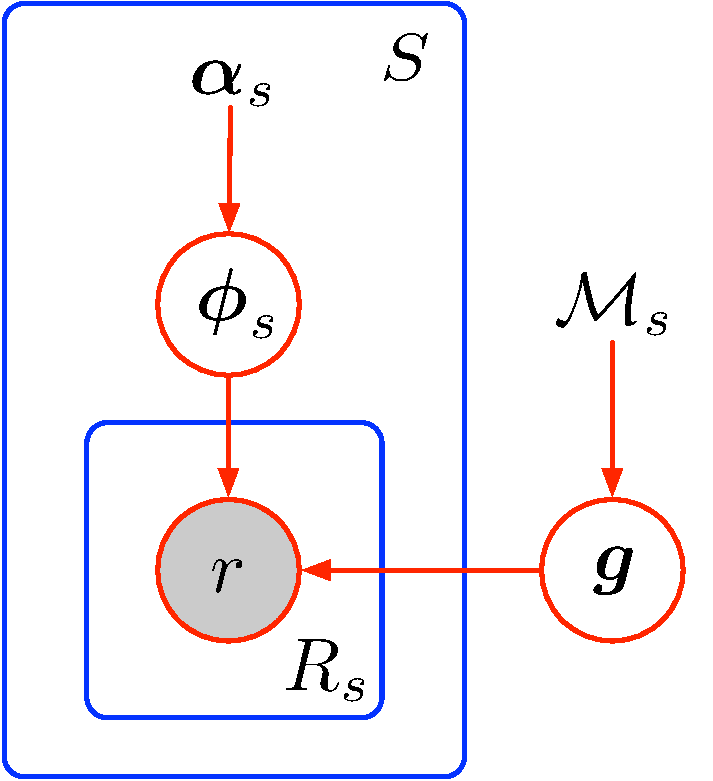
\includegraphics[width=\textwidth]{figures/subclone_model}
        \caption{}
        \label{fig:subclone}
    \end{subfigure}
    \caption{\textbf{Genotype models shown in plate notation}. \protect\subref{fig:pop} population, \protect\subref{fig:trio} trio, and \protect\subref{fig:subclone} subclone. Symbols insides circles are latent variables, observed variables are shaded. Symbols inside boxes are repeated. Symbols not inside a circle are parameters or models. Arrows define conditional relationships, red for stochastic and green for deterministic. $\theta$ is used to denote parameters for a joint genotype prior model $\mathcal{M}_p$}.
    \label{fig:genotype-models}
\end{figure*}

Genotype posterior models combine genotype prior models with genotype likelihoods. The three core genotype models currently implemented in Octopus are shown in Figure \ref{fig:genotype-models}.\\

\emph{Population genotype model.} All samples have known ploidy and copy number, so the likelihood function of a genotype $g$ given reads $\mathcal{R}$ is simply

\begin{equation*}
	p(g | \mathcal{R}) = \frac{1}{|g|} \prod_{n=1}^{|\mathcal{R}|} \sum_{i = 1}^{|g|} p(r_n | g_{i})
\end{equation*}

where $|g|$ is the ploidy and $|\mathcal{R}|$ is the number of reads. The joint genotype posterior for $S$ samples is therefore given by

\begin{equation*}
	p(\boldsymbol{g} | \boldsymbol{\mathcal{R}}, \mathcal{M}_g) \propto p(\boldsymbol{g} | \mathcal{M}_g) \prod_{s=1}^S p(\boldsymbol{g}_s | \boldsymbol{\mathcal{R}}_s)
\end{equation*}

where the genotype prior model, $\mathcal{M}_g$, is either the uniform or HWE-coalescent prior. Unfortunately, the number of genotype combinations $\boldsymbol{g}$ grows exponentially in the number of samples $S$, so we cannot evaluate the full posterior distribution in general. Therefore, other than for trivial cases, we first approximate $p(\boldsymbol{g}_s | \boldsymbol{\mathcal{R}}, \mathcal{M}_g)$ - the sample marginal genotype posterior distribution under the HWE model (without mutations), and use these marginal probabilities to select K genotype combinations $\boldsymbol{g}_i, \dots, \boldsymbol{g}_K$ (K is user defined) to evaluate under the full joint genotype model. The approximate posterior marginals are computed with Expectation Maximisation.\\

\emph{Individual genotype model.} The individual model is simply a case of the population model, without the initial approximation step; this model is always fully evaluated.\\

\emph{Trio genotype model.} The trio genotype model has the same likelihood function as the population model, but assigns prior probabilities to genotype combinations with the trio genotype prior model. Like for the population model, this model is intractable in general, so we only evaluate the posterior partially. Briefly, we evaluate approximate marginal probabilities for each sample under independence, and use these likelihoods to first combine parental genotypes, and then formulate a list of trio genotypes by combining parental combinations with offspring genotypes.\\

\emph{Subclone genotype model.} Unlike the other genotype posterior models, this model does not assume known copy number - or mixture frequency - of sample genotypes. The model assumes all read observations originate from the same underlying genotype, but may have been observed at different mixture frequencies. The mixture frequencies for each sample therefore becomes a latent variable which we infer. We use Dirichlet distributions to assign probability to mixture frequencies. Therefore, different mixture priors may be specified for each sample by controlling the concentration parameter of the respective Dirichlet distribution. The joint posterior distribution is 

\begin{equation*}
\small
p(g, \boldsymbol{\pi} | \boldsymbol{\mathcal{R}}, \boldsymbol{\alpha}, \mathcal{M}_g) \propto p(g | \mathcal{M}_g) \prod_{s=1}^S \int d \boldsymbol{\phi}_s p(\boldsymbol{\phi}_s | \boldsymbol{\alpha}_s) \prod_{r \in \boldsymbol{\mathcal{R}}_s} \sum_{i = 1}^{|g|} \boldsymbol{\phi}_{si} p(r | g_i)
\end{equation*}

where $\boldsymbol{\alpha}$ are prior concentration parameters, $\boldsymbol{\phi}$ are mixture frequencies, and $\mathcal{M}_g$ is the genotype prior model. We cannot compute this model exactly, not even partially, due to the integral over mixture frequencies. We therefore compute approximate posteriors for each latent variable using an iterative Variational Bayes (VB) procedure. Namely, we assume the posterior distribution has factorisation

\begin{equation*}
    q(\boldsymbol{g}, \boldsymbol{Z}, \boldsymbol{\phi}) = q(\boldsymbol{g}) \prod_{s = 1}^S q(\boldsymbol{Z}_s) q(\boldsymbol{\phi}_s)
\end{equation*}

where $\boldsymbol{Z}_s$ is a latent binary indicator matrix specifying read-component assignments. The associated probabilities, $p(\boldsymbol{Z}_{snk}$, are often called \emph{responsibilities} - the responsibility haplotype $k$ assumes for read $n$ in sample $s$. With this factorisation, the posterior distributions for each latent variable is conjugate with the prior; we infer Dirichlet posterior distributions. An important feature of the VB approximation is that we can easily calculate a \emph{lower bound} for the data likelihood - the model \emph{evidence}.

\subsection*{Genotype posterior marginalisation}

A common action used in Octopus is \emph{marginalisation} of genotype posterior distributions. Since all models operate on haplotypes, but ultimately allele probabilities are reported, it is important to distinguish \emph{haplotypic} genotypes from \emph{allelic} genotypes. The former is a combination of haplotypes, while the latter is a combination of alleles. Octopus is able to perform marginalisation over haplotypic genotypes as haplotypes in Octopus are explicitly represented as compound alleles.

Once we have computed the posterior distribution of haplotypic genotypes. We will often want to calculate posteriors for individual alleles. This is done by marginalising over parts of the haplotypic genotype posterior distribution that contains the allele in question, as shown in \textbf{Figure \ref{fig:marginalisation}}.

\begin{figure}[ht]
\centering
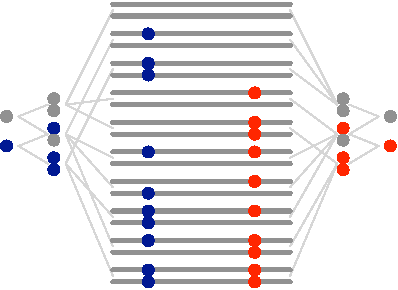
\includegraphics[width=0.5\textwidth]{figures/marginalisation}
\caption{Marginalisation of a posterior genotype distribution with two candidate variants. All haplotypic genotypes are shown in the centre. Posterior probabilities for allelic genotypes are calculated by marginalising those haplotypic genotypes that contain the allelic genotype. In turn, allele posteriors are found by marginalisation over the allelic genotype posteriors.}
\label{fig:marginalisation}
\vspace{-1.5em}
\end{figure}

A key point of marginalisation of haplotypic genotype distributions is that phase information is discarded. It is this property that allows Octopus to achieve well calibrated allelic genotype probabilities, even if phasing with surrounding segregating variants is uncertain.

\subsection*{Calling models}

Each calling model is responsible for calling variants given candidate alleles, haplotypes, and haplotype likelihoods. Although calling models are free to choose which latent variables and genotype models to use, all calling models must be able to infer posterior distributions over candidate haplotypes (for filtering), and genotypes (for phasing).\\

\emph{Individual.} Unsurprisingly, the individual calling model uses the individual genotype model for genotype inference. Haplotype posteriors are computed by marginalising over the genotype posterior distribution:

\begin{equation*}
p(h | \mathcal{R}) = \sum_{g} [h \in g]p(g | \mathcal{R})
\end{equation*}

where $h \in g$ is true if $h$ occurs in $g$ at least once. To call variants, we first calculate the posterior probability of all candidate non-reference alleles by marginalising over the genotype posterior distribution:

\begin{equation*}
p(a | \mathcal{R}) = \sum_{g} [a \in g]p(g | \mathcal{R})
\end{equation*}

where $a \in g$ is true if the $\text{any}(a \in h) \text{for} h : g$ (i.e. if $a$ occurs in any of the haplotypes in $g$). We then select alleles with posterior probability above some user-specified threshold.

Next, we identify the genotype with the greatest posterior probability (i.e. the MAP genotype). All selected alleles that appear on the MAP genotype are called variants, where the variant quality is determined by the marginalised allele posterior computed previously.

For each called allele, we then call genotypes at the loci of those alleles. In particular, for an allele $a$ we identify the alleles present in the called genotype at that loci, and once again marginalise over the genotype posterior distribution to compute the posterior probability for that local genotype. This is used for the genotype quality score.\\

\emph{Population.} Inference for the population model is similar to the individual; variant calls are made based on sample marginal posteriors.\\

\emph{Trio.} The trio calling model first infers a joint genotype posterior distribution $p(g_m, g_p, g_o | \boldsymbol{\mathcal{R}})$ with the trio genotype posterior distribution. We then infer sample marginal genotype posteriors for each sample by marginalising over the joint posterior distribution. Haplotype posteriors are calculated by integrating over the marginal posterior:

\begin{equation*}
p(h | \boldsymbol{\mathcal{R}}) = 1 - \prod_{s \in \{m, p, o\}}\sum_{g_s} [h \notin g]p(g_s | \boldsymbol{\mathcal{R}})
\end{equation*}

To calculate the probability an allele segregates in the trio, we integrate over the joint genotype posterior distribution:

\begin{equation*}
p(a | \boldsymbol{\mathcal{R}}) = 1 - \prod_{s \in \{m, p, o\}}\sum_{g_s} [a \notin g]p(g_s | \boldsymbol{\mathcal{R}})
\end{equation*}

Similarly, we calculate the posterior probability an allele is \textit{de novo} in the child:

\begin{equation*}
\small
p_{denovo}(a | \boldsymbol{\mathcal{R}}) = \sum_{g_m, g_p, g_o \in \boldsymbol{g}} [a \notin g_m \land a \notin g_p \land a \in g_o] p(g_m, g_p, g_o | \boldsymbol{\mathcal{R}})
\end{equation*}

Finally, we find the MAP genotype combination using the joint genotype posterior distribution, and only call variants that are included in this trio. \\

\emph{Cancer.} The cancer calling model is intended to detect somatic mutations in a set of tumour samples from a single individual. The set of samples may also include a sample that is not expected to contain somatic mutations - a normal or control sample. We attempt to model three expected observations that result from tumour biology and experimental protocol; for a given loci, we expect: 

\begin{enumerate}[i]
	\item There are no somatic mutational events; reads are generated from a clean germline.
	\item Copy number changes have occurred, but no somatic mutations.
    \item Somatic mutations have occurred, \emph{and} possibly copy number changes.
\end{enumerate}

Each of these three cases is modelled by fitting a unique genotype posterior model:

\begin{enumerate}[i]
	\item The individual model with any germline genotype prior model (all read observations are merged): $\mathcal{M}_{ind}$.
	\item The subclone model with the \emph{germline} genotype prior model: $\mathcal{M}_{CNV}$.
    \item The subclone model with the \emph{cancer} genotype prior model: $\mathcal{M}_{somatic}$.
\end{enumerate}

The posterior probability for each model is calculated using Bayes theorem:

\begin{equation*}
    p(\mathcal{M}_{x} | \boldsymbol{R}) \propto p(\mathcal{M}_{x}) p(\boldsymbol{R} | \mathcal{M}_{x})  
\end{equation*}

where $p(\boldsymbol{R} | \mathcal{M}_{x})$ is the \emph{evidence} for model $x$.

For the somatic case, $\mathcal{M}_{somatic}$, we must also infer the number of segregating somatic haplotypes. To do this we start by assuming a single somatic haplotype, and incrementally add more while the evidence for the model is the greatest observed so far, up to a user defined limit.

For inference, we must marginalise over models. For example, we calculate posteriors for germline genotypes by marginalisation:

\begin{align*}
p(g | \boldsymbol{\mathcal{R}}) &= p(\mathcal{M}_{ind} | \boldsymbol{\mathcal{R}}) p(g | \mathcal{M}_{ind}) \\
&+ p(\mathcal{M}_{CNV} | \boldsymbol{\mathcal{R}}) p(g | \mathcal{M}_{CNV}) \\
&+ p(\mathcal{M}_{somatic} | \boldsymbol{\mathcal{R}}) p(g | \mathcal{M}_{somatic})
\end{align*}

\noindent where $p(g | \mathcal{M}_{somatic}) = \sum_{\tilde{g} s.t. g \in \tilde{g}} p(\tilde{g} | \mathcal{M}_{somatic})$ (i.e. marginalise over cancer genotypes that contain the matching germline component).

The posterior probability of an allele $a$ segregating in the germline is then:

\begin{equation*}
p(a | \boldsymbol{\mathcal{R}}) = \sum_{g s.t. a \in g} p(g | \boldsymbol{\mathcal{R}})
\end{equation*}

Germline candidates are called if the posterior is above a user defined threshold, and if the candidate is present in the called germline genotype. If the candidate is not above the user-defined threshold, it is added to a list of candidate somatic candidates.

To calculate the posterior probability an allele $a$ is a real somatic mutation, we need to marginalise over $\mathcal{M}_{somatic}$. First we calculate the posterior mass for \emph{credible} somatic frequencies. Supposing that we inferred a model with $K$ somatic haplotypes, we assign probability to each somatic haplotype $k = 1 \dots K$ if it occurs as a frequency above some user defined threshold, $\tau$

\begin{equation*}
p(\boldsymbol{\phi}_{sk} > \tau | \mathcal{M}_{somatic}) = \int_{\tau}^1 \text{Beta}(\alpha_{P + 1}, \sum_{i = 0}^{P} \alpha_i)
\end{equation*}

where the equality holds since the posterior distribution for $\boldsymbol{\phi}_{s}$ is Dirichlet. The overall credible somatic mass $\lambda_{s}$ is then calculated with

\begin{equation*}
\lambda_{s} = 1 - \prod_k 1 - p(\boldsymbol{\phi}_{sk} > \tau | \mathcal{M}_{somatic})
\end{equation*}

Finally we set $\lambda = 1 - \prod \lambda_s$. We then calculate the posterior probability that an allele is a somatic mutation by marginalisation:

\begin{equation*}\small
p_{somatic}(a | \boldsymbol{\mathcal{R}}) = \lambda(1 - \prod_s \sum_{a \notin \tilde{g}.germline \land a \in \tilde{g}.somatic : \tilde{g}}p(\tilde{g} | \boldsymbol{\mathcal{R}}, \mathcal{M}_{somatic}))
\end{equation*}

\noindent If this probability is greater than some user-defined threshold, we proceed to call somatic mutations.

For both called germline and somatic mutations, we also calculate the probability that the variant segregates regardless of classification in a similar fashion. \\

\emph{Polyclone.} The polyclone calling model is similar to the cancer calling model without the third somatic mutation model; It compares the individual genotype model with haploid genotypes, with the subclone genotype model. The number haplotypes in the latter case it determined iteratively by comparing model evidences.

\subsection*{Probabilistic phasing}

Although each caller implements different genotype models, each is required to infer the \emph{marginal} posterior probability of genotypes for each sample. This posterior distribution is used to infer physical phasing of called variant sites. Direct read data is not required as all information available from the reads, in addition to any prior information, is already contained in the posterior distribution. The advantage of this approach is exemplified when calling trios as the genotype prior can be strongly informative about phase due to identity by decent. The method applies to genotypes of arbitrary zygosity and is therefore applicable to non-diploid samples.

\begin{figure}[ht]
    \centering
    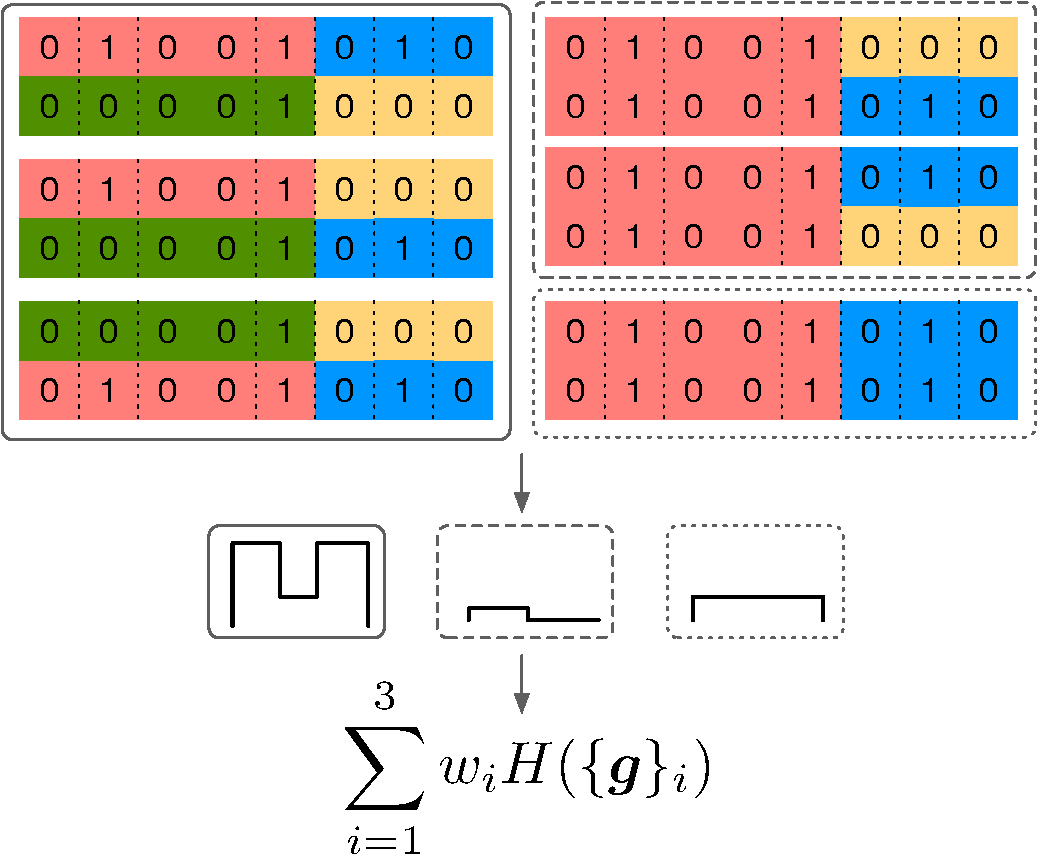
\includegraphics[width=0.5\textwidth]{figures/phasing}
    \caption{A subset of phase complement sets for three candidate variants used to calculate phase scores.}
    \label{fig:phasing}
\end{figure}

Samples are phased independently; the marginal genotype posterior distribution for each sample is used for phasing (\textbf{Figure \ref{fig:phasing}}). First, all genotypes in the domain of the posterior distribution are partitioned into \emph{phase complement} sets. All genotypes in a phase complement set share exactly the same alleles, although they may appear on different haplotypes. There is only one such partitioning possible for any set of genotypes. We calculate the entropy of each set with respect to the normalised posterior probabilities of the genotypes contained in the set. A low entropy implies little uncertainty in the phase of the alleles present in the set. To account for uncertainty in the samples genotype, we marginalise over all phase complement sets by taking the weighted sum of each sets entropy, where the weight for each set is the sum of the unnormalised posterior probabilities. We termed this weighted average a \emph{phase score}.

\begin{equation*}
    \text{PS}(\boldsymbol{g} | \mathcal{R}_s) = \sum_j \tau_j H\left(\left[\frac{p(g_{j0} | \mathcal{R}_s)}{\tau_j}, ..., \frac{p(g_{jm}| \mathcal{R}_s)}{\tau_j}\right]\right)
\end{equation*}

Lower phase scores indicate less ambiguous phasing, even if there is high uncertainty in the samples genotype. If the phase score for a set of genotypes is lower than a given threshold the region is considered phased, otherwise, each genotype in the set can be broken into two parts which results in two unphased sets of partial genotypes. The phase scores of these two partial sets is never greater than the phase score of the original genotype set. The phasing algorithm therefore iteratively finds the smallest set of breakpoints such that the partial genotype sets defined by those breakpoints are all phased.

\subsection*{Variant filtering}

As with any model, there are some error modes that are not well captured by Octopus’ calling models which can lead to false inferences. For example, Octopus assumes read sequencing and mapping errors are independent which is not true in general. To identify false calls due to model error, we developed classifiers to filter Octopus’s raw calls using statistics, called \emph{measures} in Octopus, that may be derived directly from the input read data.

\emph{Hard filtering.} Hard filters are Boolean expressions where the terms of the expression are comparison operations. Currently, only \emph{or} binary operations are permitted; if any of the individual operations is true then the call is filtered. However, it would not be difficult to extend this to more general Boolean expressions. Different filter expressions can be specified for germline variant, \textit{de novo}, somatic, and homozygous reference calls.

\emph{Random forest filtering.} Octopus uses the Ranger library \cite{RN564} for random forest classification. We allow different random forests to be used for germline and somatic calls.

\emph{Random forest training.} We trained three random forests, one for germline variants, one for somatic mutations with normal pairs, and another for somatic mutations without normal pairs. For the germline forest we used high and low coverage NA12878 BAMs from the 1000G project, and a NA12878 read set from the Garvan institute (not the same as that used for the Precision FDA Consistency test). For the somatic forests we used chromosome X of the synthetic skin tumour. We note that it is possible to train a single random forest for both paired and unpaired somatic, or even a single random forest for all types of calls. However, it usually better to take advantage of known structure in the data where possible.

\subsection*{BAM realignments}

Octopus is capable of producing realigned BAM files that provide further evidence of a calls reliability. These BAM files are especially helpful in cases where there are complex indel variants and the input alignments are significantly different from the alignments supported by the called haplotypes. For each read, there are four steps:

\begin{enumerate}
	\item Identify the called haplotype where the read originated from.
	\item Align the haplotype to the reference sequence.
	\item Align the read to the haplotype (mismatches due to sequencing or calling errors).
	\item Merge the two alignments to obtain a single alignment to the reference.
\end{enumerate}

For the first step, we use the called haplotype that has the maximum likelihood of generating the read. If there are more than one haplotype that have equal likelihood, then we call the read \emph{ambiguous}. For the purpose of BAM realignment, ambiguous are assigned randomly to one of the equally well supported haplotypes. The second step is trivial in Octopus since haplotypes are defined explicitly by alleles that are reported in the VCF output. The third step is also trivial; we just use the Viterbi alignment found from calculating the maximum likelihood in the first step. The final step is tricky if the alignment found in the third step has indel mismatches. We always try to report an alignment that has the fewest number of CIGAR operations.

Since Octopus makes a hard choice of called haplotype in the first step, it is also possible to report this information in the BAM output. One way to do this would be to tag the read with this information. While we will look to implement this in the future, another simple way is to produce separate BAM files for each of the called haplotypes in the sample. Octopus is also capable of producing these 'split' realigned BAMs.

\subsection*{Synthetic tumours}

To generate synthetic tumour BAM files we followed a similar approach to Ewing et al. \cite{RN147} with important differences. First, we obtained unmapped reads from the GIAB's NA12878 high coverage HiSeq 2500 set ($\sim 300$x total). In contrast to Ewing et al., we felt it was important to use a sample with a well characterised germline profile. From the high coverage set, we partitioned the reads into three non-overlapping subsets, keeping reads sequenced derived from the same library together, such that for each subset would have sufficient reads to generate a 30x 'normal' BAM and a 60x 'tumour' BAM. This ensures all reads used for evaluation are unique, but maintains realistic sequencing conditions.

For each of the three 'tumour' BAMs, we then performed a haplotype-based read assignment and realignment. First, for each tumour BAM, we used high quality NA12878 phased germline variants called with Octopus (GIAB F1 0.9995) to assign each each read a single called haplotype with the maximum likelihood alignment score. Reads supporting heterozygous loci were assigned to separate sets and reads supporting homozygous sites (reference or alternative) were assigned to a third set. This results in three \emph{bona-fide} haploid sub-BAMs. We then realigned all reads in each of these sub-BAMs in a variant aware manner (i.e. to the haplotype they support). The purpose of the assignment step is to ensure spike in mutations fall on the same germline haplotype. The realignment step is to ensure consistency of spike in location. Neither of which are guaranteed by the method described in Ewing et al due to limitations with BAMSurgeon. In summary, this procedure results in three unique BAM subsets, each of which should be haploid and contain almost no alignment errors.

We then simulated sets of somatic mutations for each of the three 'tumour' BAMs. In contrast to Ewing et al. which used randomly generated mutations, we generated somatic mutations by sampling putative real somatic mutations called by the PCAWG consortium. In particular, we sampled PCAWG calls from a single tumour type for each of our three 'tumours' (breast, skin, and colorectal) in such a way to achieve a particular genome-wide mutation rate ($2e-6$, $1e-5$, and $1e-4$ respectively), which were selected from the upper expected range for each tumour type \cite{RN86}. We sampled each PCAWG mutation independently in order to maintain the local mutation characteristics of each tumour type. For each sampled mutation, we randomly assigned a spike in variant allele frequency from 0.05 to 1.0 (from 20 equally spaced bins), in essence creating 20 'subclones'. Although this frequency distribution is unlikely to be biologically realistic, we used this approach to better evaluate the performance of each algorithm across a range of allele fractions. Each sampled somatic mutation was then randomly assigned to a germline haplotype (all chromosomes in this case as NA12878 is female).

We used a slightly modified version of BAMSurgeon to spike in somatic mutations into our haploid BAMs. The VAF used for the third BAM, which should in principle contain reads from both parental haplotypes, was always half that used for the desired VAF. For example, if a VAF of 1.0 was chosen for a mutation assigned to haplotype 1, the mutation would be spiked in at frequency 1.0 in the first BAM, at 0.5 in the third BAM, and not at all in the second, which results in a overall frequency of 0.5. The main modification we needed to make to BAMSurgeon was to ensure any 'pad' sequence used for deletion spike-ins, comes from the observed germline haplotype, rather than the reference. We also needed to make minor modifications to handle our split BAM files, which are not likely to contain properly paired reads.

Finally, we merged each of the three somatic spiked sub-BAMs, and extracted paired FASTQ files. These spiked 'tumour' FASTQ files are used for each somatic mutation calling pipeline. We emphasise that the FASTQ extraction step removes all alignment information, so any advantage that Octopus, or any other caller, may have gained from the realigned reads is lost.

\subsection*{Data availability}

Octopus source code and documentation is available on Github under the MIT license (\url{https://github.com/luntergroup/Octopus}).

The trained random forests use for benchmarks can be accessed from Google Cloud (\url{https://storage.googleapis.com/luntergroup/Octopus/forests}).

The synthetic tumour and paired normal FASTQs are available from Google Cloud (\url{https://storage.googleapis.com/luntergroup/syntumour}.)

\subsection*{Author contributions}

D.C and G.L designed the algorithm and wrote the manuscript. D.C implemented the algorithm and performed the the evaluation. D.W provided data for the synthetic tumours and critically reviewed the manuscript. 

\subsection*{Competing interests}

G.L is a co-founder of Genomics Plc.  

\end{document}